\chapter{Experimentos computacionales}
\label{sect:problemresults}

En este capítulo ponemos a prueba el modelo resultante del capitulo \ref{sect:problemresolution}. Para empezar estudiamos el comportamiento del modelo frente a perturbaciones en alguno de sus parámetros específicos del problema, es decir modelado de la transferencia de demanda, presupuesto y tecnologías de ciclovías, sobre la red de Sioux-Falls de manera de poder realizar pruebas en tiempo razonable. En particular, analizamos los resultados respecto a la demanda transferida total y a las decisiones que se toman sobre las ciclovías a construir. Luego aplicamos el modelo a una instancia de tamaño realista que modela la ciudad de Montevideo. Antes de presentar los resultados, discutimos el criterio con el que elegimos los valores de costos de construcción de las diferentes tecnologías de ciclovía, costos de usuario por tecnología, funciones de transferencia de demanda y valores de presupuesto.

\section{Especificación de datos}
\label{sect:dataspecification}

Nuestro problema requiere la disponibilidad de parámetros que en la práctica no son fáciles de estimar de forma realista como los costos usuario y construcción por tipo de tecnología y transferencia de demanda en función del costo de usuario. En esta sección definimos algunos criterios que utilizamos para especificarlos en base a trabajos de la literatura. En la siguiente, analizamos qué efectos tienen las perturbaciones sobre las soluciones.

La cantidad y tipos de tecnologías de ciclovía varían de un contexto a otro tanto en su disponibilidad como en sus costos y por lo tanto es difícil estimar estos últimos de manera general sin llegar a un análisis caso a caso. Por ejemplo en la ciudad de Montevideo podemos encontrar tres tipos \footnote{Mapa interactivo: \url{https://montevideo.gub.uy/mapa-montevideo-en-bici}}: el más básico consiste en imponer un límite superior de velocidad para los vehículos automotores (30 km/h) y cartelería resaltando cierta calle o zona como habilitada para el tránsito en bicicleta. Un segundo tipo consiste en utilizar una fracción de la calle como senda específica para bicicletas que puede ir en uno o ambos sentidos. Y el tercer tipo consta de una bicisenda construida específicamente para bicicletas generalmente en canteros y parques.

Los costos de construcción pueden variar según la ubicación y tipo de ciclovía, congestión del área de la ciudad y su afectación por las obras, precios de insumos externos como el petróleo y cuestiones logísticas como reubicación de paradas de ómnibus y señales de tránsito, entre otros aspectos. Se puede encontrar información al respecto en el análisis \cite{typicalcostsofcylcing} que presenta diversos tipos de tecnologías y los principales factores que afectan el costo de construcción como trabajo dentro de un programa de incentivo del transporte en bicicleta en Inglaterra. En base a dicho trabajo simplificamos y generalizamos el cálculo de los cotos de construcción para cada tipo de tecnologías de la siguiente manera: la tecnología de tipo $i + 1$ cuesta el doble que la tecnología de tipo $i$. Esto también es consistente con la información disponible para la ciudad de Montevideo \footnote{Información obtenida por comunicación personal con la Intendencia de Montevideo.}. Entonces, sean $l_a$ el largo del arco $a \in A$ y $CC_i$ el costo de construcción de la tecnología $i \in I$ por unidad de distancia, los costos de construcción por tecnología y arco quedan: $H_{ai} = l_a CC_i, \forall a \in A, i \in I$; donde $CC_i = 2 * CC_{i-1}, \forall i > 2$; $CC_1 = 1$ y $CC_0 = 0$.

Por otro lado, los costos de usuario de atravesar un arco varían en la práctica dependiendo de factores como ancho de la vía, pavimento, volumen y velocidad del tránsito, entre otros, que a su vez se ponderan por el largo del arco. En el documento \cite{blos2007} podemos encontrar el concepto de {\it Bicycle Level of Service} (BLOS), muy utilizado en la literatura, que agrupa estas consideraciones bajo un único valor. Para el cálculo del BLOS se tienen en cuenta los distintos aspectos que cuantificados en indicadores, son luego utilizados en una fórmula para calcular el puntaje de BLOS que se estratifican en 6 niveles del A al F.

Los aspectos que se consideran son los siguientes:

\begin{enumerate}
  \item{Ancho promedio de la banquina, presencia de ciclovía, porcentaje de la vía ocupada por estacionamiento}
  \item{Límite de velocidad de vehículos motorizados}
  \item{Volumen promedio de los vehículos motorizados}
  \item{Porcentaje de tránsito pesado (camiones)}
  \item{Condición del pavimento}
\end{enumerate}

\begin{table}[h!]
  \centering
  \begin{tabular}{cccc}
    \toprule
      Nivel & Puntaje BLOS & Tecnología & \shortstack{Proporción de mejora \\ sobre costo base} \\
    \midrule
      A     & $\leq 1.5$   & 5              & 0,4   \\
      B     & 1,5-2,5      & 4              & 0,52  \\
      C     & 2,5-3,5      & 3              & 0,64  \\
      D     & 3,5-4,5      & 2              & 0,76  \\
      E     & 4,5-5,5      & 1              & 0,88  \\
      F     & > 5,5        & 0              & 1     \\
    \bottomrule
  \end{tabular}
  \caption{Niveles de servicio definidos en el BLOS, menor puntaje BLOS representa mejores condiciones para el usuario. Para cada nivel definimos un tipo de tecnología y su correspondiente proporción de mejora sobre la tecnología base.}\label{table:blosscores}
\end{table}

En esta tesis nos enfocamos en la planificación estratégica de una red ciclovías sin asumir aspectos detallados para su diseño por lo tango ignoramos algunos factores tomados en cuenta para el cálculo del BLOS. Mediante la construcción de infraestructura de ciclovía solo podemos mejorar alguno de los siguientes aspectos: límite de velocidad de vehiculos motorizados, presencia de ciclovías y condiciones del pavimento.

Tomando como base el puntaje de BLOS estratificado de la Tabla \ref{table:blosscores}, siguiendo el cálculo en \cite{baya2021}, podemos traducir de forma aproximada los puntajes de BLOS a proporción de mejora sobre la tecnología base o red de calles utilizando la función $C_{infra}(i) = {28 - 3 (i + 1) \over 25}$ donde $i \in I = \{0,1,2,\ldots\}$ es el tipo de tecnología. Suponiendo que el nivel F de la escala de BLOS corresponde a tecnología base (o tecnología 0), la proporción de mejora de las tecnologías A-E correspondientes a los tipos de tecnologías 5,4,3,2 y 1 respectivamente se pueden observar en la misma tabla.

Incurrimos a la simplificación de considerar, al definir una instancia, la cantidad $T$ de tipos tecnologías posibles a utilizar y no cuáles, de manera que los tipos de tecnología utilizables sean $I = \{0,.., T - 1\}$. Dada una instancia del problema, llamamos $m$ a la proporción de mejora máxima que puede dar la mejor tecnología de entre las disponibles, es decir $m = C_{infra}(T - 1)$. El valor $m$ es de utilidad al definir las funciones de transferencia de demanda como veremos a continuación.

Respecto al comportamiento de los usuarios, suponemos que la demanda de todos los pares origen-destino se comporta de igual manera, lo cual tiene sentido al considerar una población determinada. Esto reduce la necesidad de especificar $|OD|$ funciones de transferencias de demanda a una sola. Es decir, para cada par origen destino $k$, tenemos que $f_k(w_k) = f({w_k \over S^{best}_k})d_k$, donde $d_k$ es la demanda máxima que se puede transferir, $S^{best}_k$ es el costo del camino más corto sobre la tecnología base y $f: [m, 1] \rightarrow [0, 1]$ modela la proporción de demanda transferida en función de la proporción del nuevo costo sobre el costo base $S^{best}_k$.

Partimos de \cite{shwe2014} en el que analizando una extensiva encuesta realizada en varios países aproxima la proporción de viajes hechos en bicicleta y el largo de infraestructura de ciclovía per cápita en la ciudad a una relación lineal. Tomando este resultado, utilizamos una función lineal decreciente como función de transferencia de referencia. Como alternativa, en \cite{ortuz2011} se menciona que el comportamiento de la demanda al momento de decidir entre dos modos se comporta como una función con forma de S, logística o sigmoide, por lo que también consideramos una función logística en nuestras pruebas. Por completitud analizamos otras funciones que podrían considerarse razonables: una con concavidad estrictamente positiva y otra con concavidad estrictamente negativa en el intervalo $[m, 1]$. La definición explícita se encuentra en la Sección \ref{sect:fspecification}.

Establecer valores de presupuesto realistas depende altamente de las condiciones políticas y económicas de cada localidad. Podemos encontrar en \cite{rios2015} y \cite{shwe2014} que factores de cubrimiento de la red de ciclovías en una ciudad de entre 10\% y 40\% del total de la red de calles de una ciudad están dentro de los parámetros normales. Seguimos este enfoque y especificamos el presupuesto como porcentaje del costo total de construir una infraestructura de ciclovía en toda la red tomando como referencia el costo de la tecnología 1, es decir la tecnología especializada más básica que sigue a la red de calles. Dado nuestro método para el cálculo de los costos de los tipos de tecnologías, esto implica que un presupuesto del 40\% es suficientemente para cubrir 20\% solo con la tecnología de tipo 2, 10\% solo con la tecnología de tipo 3; y en general un factor de $F\%$ cubre ${F \over {2^{i - 1}}}\%$ de la tecnología $i \in \{1,..,5\}$.

Finalmente, usamos el largo de los arcos como costo de usuario y costo de construcción de la tecnología 1. Esto nos da una medida suficientemente simple y general como para usar en cualquier instancia.

\section{Especificación de funciones de transferencia de demanda}
\label{sect:fspecification}

Las funciones de transferencia de demanda probadas fueron cuatro, ver Figura \ref{fig:fcatalog}. Si bien las funciones fueron creadas para este trabajo, las versiones lineal y logística están basadas y son consistentes con los trabajos de \cite{shwe2014} y \cite{ortuz2011} respectivamente. Las versiones con concavidad negativa y positiva fueron creadas para complementar el estudio y están compuestas de funciones logísticas desplazadas de manera de lograr la concavidad deseada en el intervalo $[m, 1]$.

Las expresamos parametrizadas por $m$, correspondiente a la proporción de mejora máxima alcanzable por la mejor tecnología, ya que es el mínimo valor que tiene sentido. Definimos las funciones en $[m, 1] \rightarrow [0, 1]$ de la siguiente manera:

\begin{definition}
  Lineal
  \begin{align}
      f(x) = {x -1 \over m - 1}
  \end{align}
\end{definition}

\begin{definition}
  Logística
  \begin{align}
      f(x) = {1 \over 1 + e^{2k_m(x - ({1 + m \over 2}))}}
  \end{align}
\end{definition}

\begin{definition}
  Concavidad negativa.
  \begin{align}
      f(x) = {2 \over 1 + e^{k_m(x - 1)}} - 1
  \end{align}
\end{definition}

\begin{definition}
  Concavidad positiva.
  \begin{align}
      f(x) = {2 \over 1 + e^{k_m(x - m)}}
  \end{align}
\end{definition}

El parámetro $k_m$ determina la pendiente de las funciones basadas en la función logística y es utilizado para que los valores funcionales en los extremos de $(m, 1)$ estén cerca de $1$ y $0$ respectivamente. Fue determinado de manera experimental y se calcula como $k_m = {3 \over 1 - m}$. Al utilizar estas funciones fue necesario normalizar el codominio de manera que abarque el intervalo $[0, 1]$ dado que el parámetro $k_m$ no garantiza que esto suceda.

\begin{figure}[h!]
  \centering
  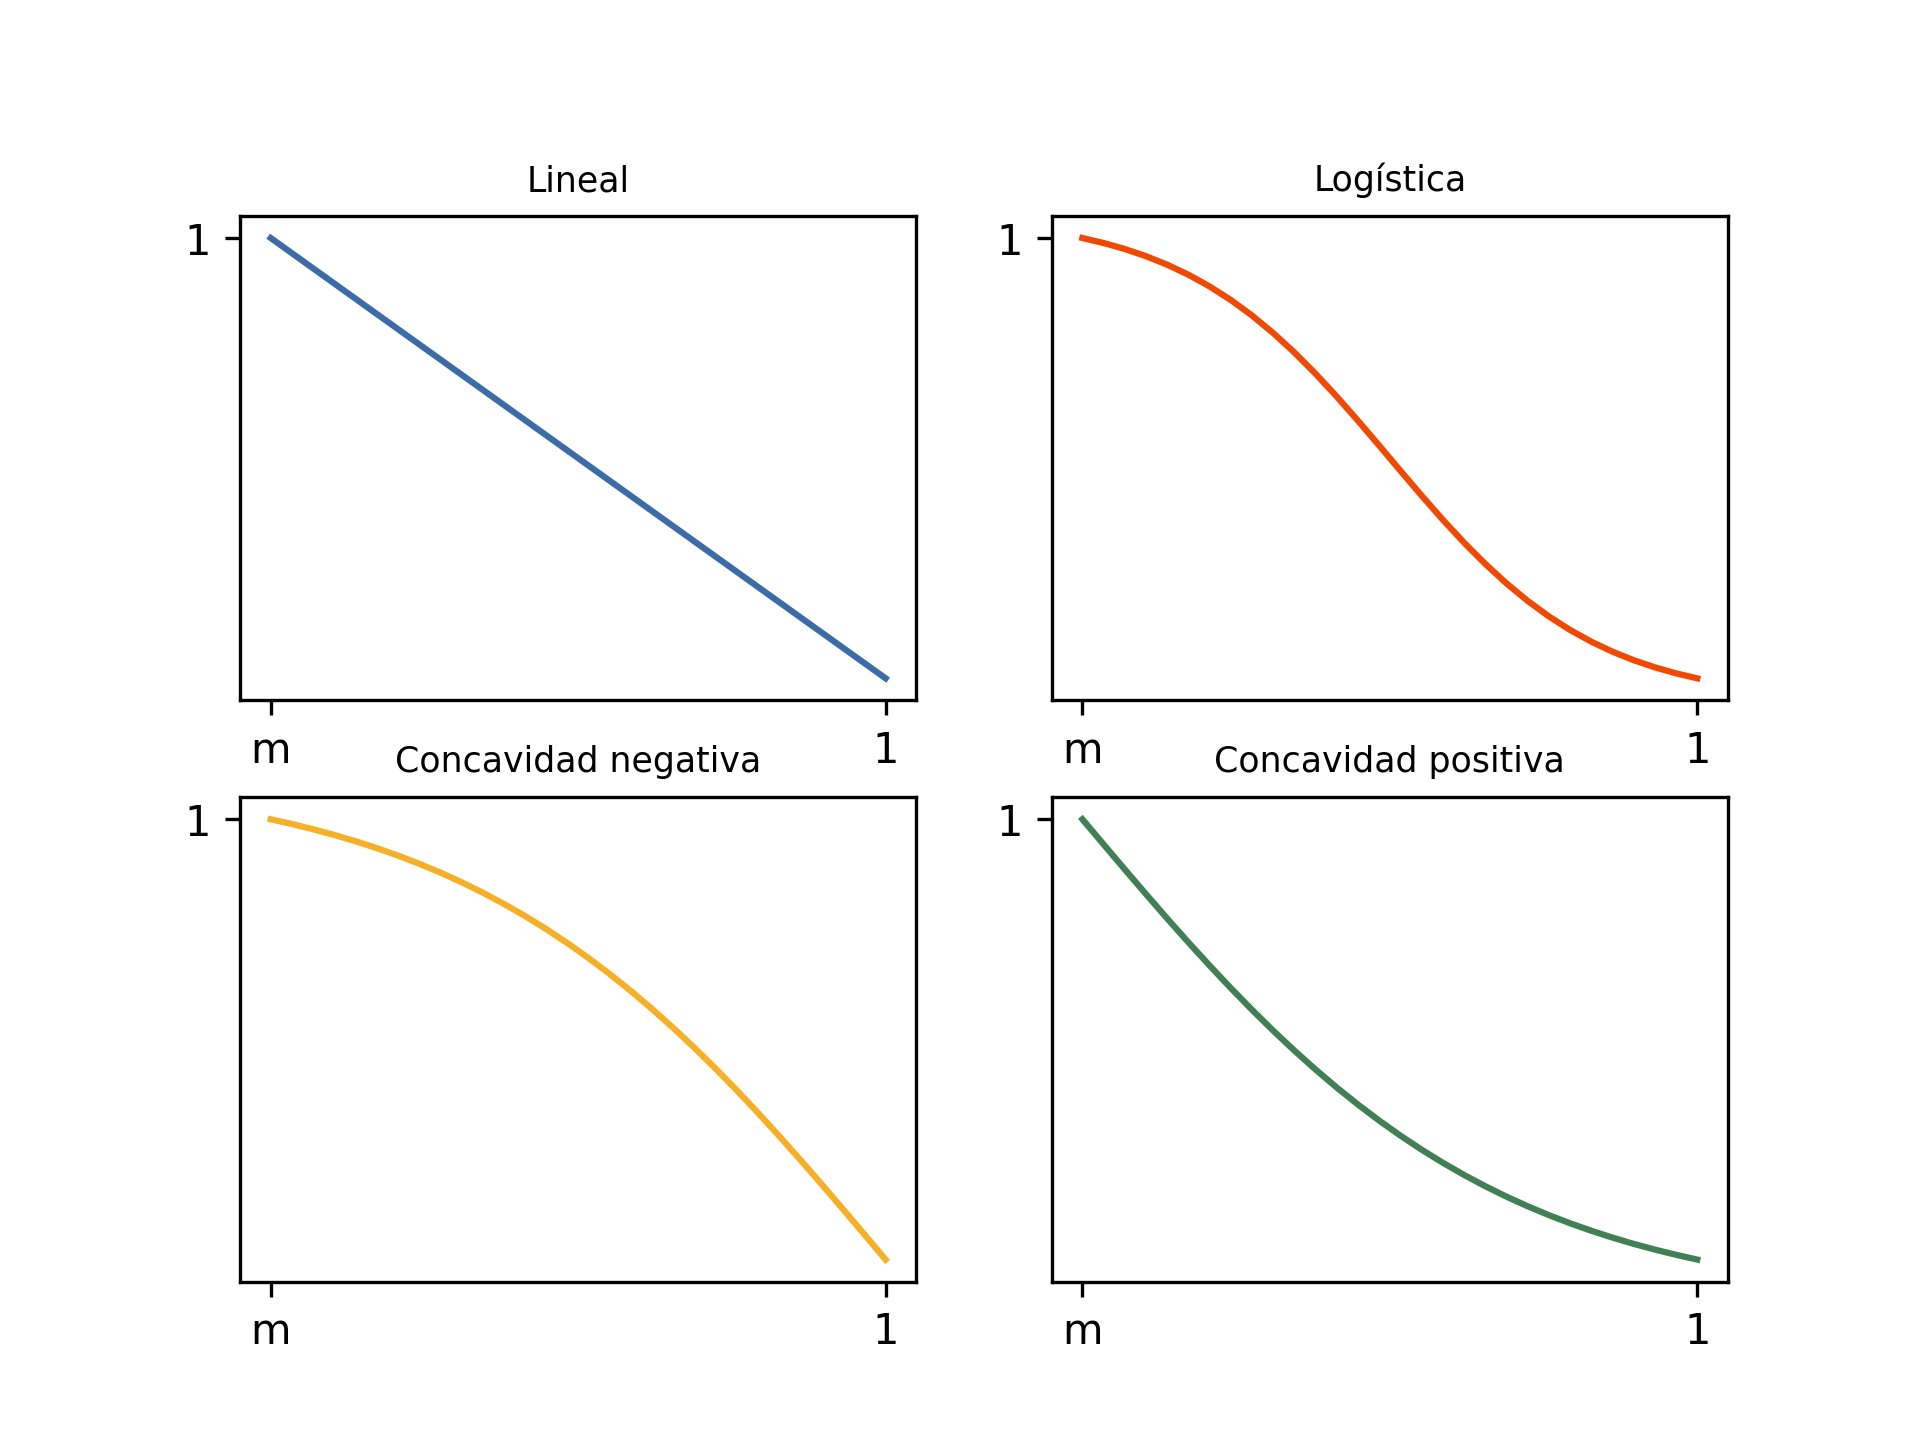
\includegraphics[width=10cm]{../resources/f_catalog.png}
    \caption{Catálogo de funciones usadas para modelar la transferencia de demanda a la bicicleta. El valor de $m$ varía según la tecnología de ciclovía utilizada y equivale a la proporción mínima alcanzada por la mejor tecnología utilizada, es decir $m = min_{i \in I} \{ C_{infra}(i) \}$.}
  \label{fig:fcatalog}
\end{figure}

\section{Análisis de sensibilidad}

Estudiamos el comportamiento del modelo frente a perturbaciones en alguno de sus parámetros. Utilizamos la red de Sioux-Falls nuevamente dado que es de un tamaño manejable para realizar todas las ejecuciones en tiempo razonable. Las perturbaciones las realizamos sobre los parámetros específicos del problema, dejando los datos de la red y matriz de demanda fijos. Estos son: puntos de quiebre, funciones de transferencia de demanda y presupuesto. Observar que los parámetros estudiados son de distinta naturaleza: mientras que los primeros dos son relativos al modelado del comportamiento de la demanda el último es una decisión exclusiva de la entidad planificadora. La matriz de demanda se toma de \cite{Liu2019}, con 22 pares origen-destino. Los datos de la red y matriz de demanda se encuentran en el Apéndice \ref{sect:siouxfallsdata}.

\FloatBarrier
\subsection{Perturbaciones}

Uno de nuestros objetivos es determinar cuáles son las perturbaciones, más allá de un incremento en el presupuesto, que resultan en mayores valores de demanda transferida total. Por un lado, la cantidad de tipos de tecnologías disponibles es determinante respecto a la mejora alcanzable en los caminos. Es de esperar que el modelo decida utilizar mejores tecnologías en los arcos con mayor flujo de demanda, tanto como el presupuesto y tipos de tecnologías disponibles lo permitan. En principio no hay razón para limitar este número a un valor distinto del mayor valor posible, a menos que el deterioro en el tiempo de ejecución lo haga necesario. Respecto a los puntos de quiebre, esperamos que una mayor granularidad aporte positivamente a nuestro objetivo, aunque, al igual que la cantidad de tipos de tecnologías, tendremos cuidado con deterioro en el desempeño.

Como instancia de referencia consideramos la red de Sioux-Falls y matriz de demanda antedicha y el siguiente conjunto de parámetros en base a la discusión de la sección anterior:

\begin{description}
  \item[Tecnologías de ciclovía]: 5 tipos de tecnologías además de la base.
  \item[Puntos de quiebre]: Función lineal de transferencia de demanda con 5 puntos de quiebre.
  \item[Presupuesto]: Factor de presupuesto del 80\%.
\end{description}

Las perturbaciones las realizamos sobre el conjunto de parámetros de la instancia de referencia aplicando una o dos perturbaciones por vez en lugar de ejecutar todas las posibles combinaciones de parámetros perturbados, ya que esto implicaría una mayor cantidad de instancias a estudiar.

En primer lugar analizamos la sensibilidad respecto al factor de presupuesto. Los valores utilizados son: 10\%, 80\%, 160\% y 320\%. El objetivo es observar si se cumple la simple intuición de que siempre a mayor presupuesto se obtienen mejores resultados y cómo es el comportamiento de la demanda transferida total respecto a los incrementos de presupuesto. También analizamos el efecto que tiene la cantidad de puntos de quiebre en los resultados, utilizando 5 y 20 puntos para cada presupuesto.

Luego, comparamos el resultado de aplicar diferentes funciones de transferencia de demanda y cómo afecta el hecho de utilizar distintas cantidades de puntos de quiebre. Utilizamos 5, 20 y 50 puntos de quiebre junto a las cuatro funciones mencionadas en la sección anterior (\ref{sect:dataspecification}). Definimos los puntos de manera que sean equidistantes en el codominio, es decir, si hay N puntos, de un punto al siguiente se obtiene una mejora de aproximadamente ${1 \over N - 1}$ en la proporción de demanda transferida.

Como resultado tenemos 36 instancias cuya representación pre simplificaciones en solver CPLEX son matrices que van desde un tamaño de 12597x12310 con 562 variables binarias hasta 14487x14290 con 1552 variables binarias.

\FloatBarrier
\subsection{Resultados}

Las instancias fueron ejecutadas con el solver CPLEX versión 12.8.0.0 en su configuración por defecto sobre una máquina Intel Core i9-9900K con 64GiB de RAM. Los resultados generales de las ejecuciones se encuentran en la Tabla \ref{table:sensibilityresults} y los datos sobre el uso del presupuesto, que luego comentaremos, en la Tabla \ref{table:sensibilitybudgetusage}.

Se puede observar que a mayor cantidad de puntos de quiebre, fijando la función de transferencia de demanda y el presupuesto, obtenemos mayor transferencia de demanda. Esto tiene sentido ya que la función de transferencia es representada de manera más precisa. También vemos que variar la cantidad de puntos de quiebre parece hacer variar el tiempo de ejecución en algunos casos, sin poderse determinar una relación general entre la cantidad y la complejidad resultante pero si podemos ver que fijando los otros parámetros y aumentando la cantidad de puntos de quiebre la complejidad aumenta. Por otro lado, observamos un fuerte impacto del modelado del comportamiento de la transferencia de demanda, es decir de cuál función se utiliza, sobre la demanda transferida. Esto nos confirma que es un aspecto importante del modelado, si bien las funciones consideradas en este caso pueden haber sido poco realistas o exageradas en sus curvaturas. Finalmente, vemos que la demanda transferida en función de la cantidad de presupuesto, fijando cantidad de puntos de quiebre y función de transferencia de demanda, parece crecer según la curva de la Figura \ref{fig:demandtransferbybudgetlinear} con concavidad negativa, lo que implica que el beneficio marginal de aumentar el presupuesto es cada vez menor.

\begin{figure}[h!]
  \centering
  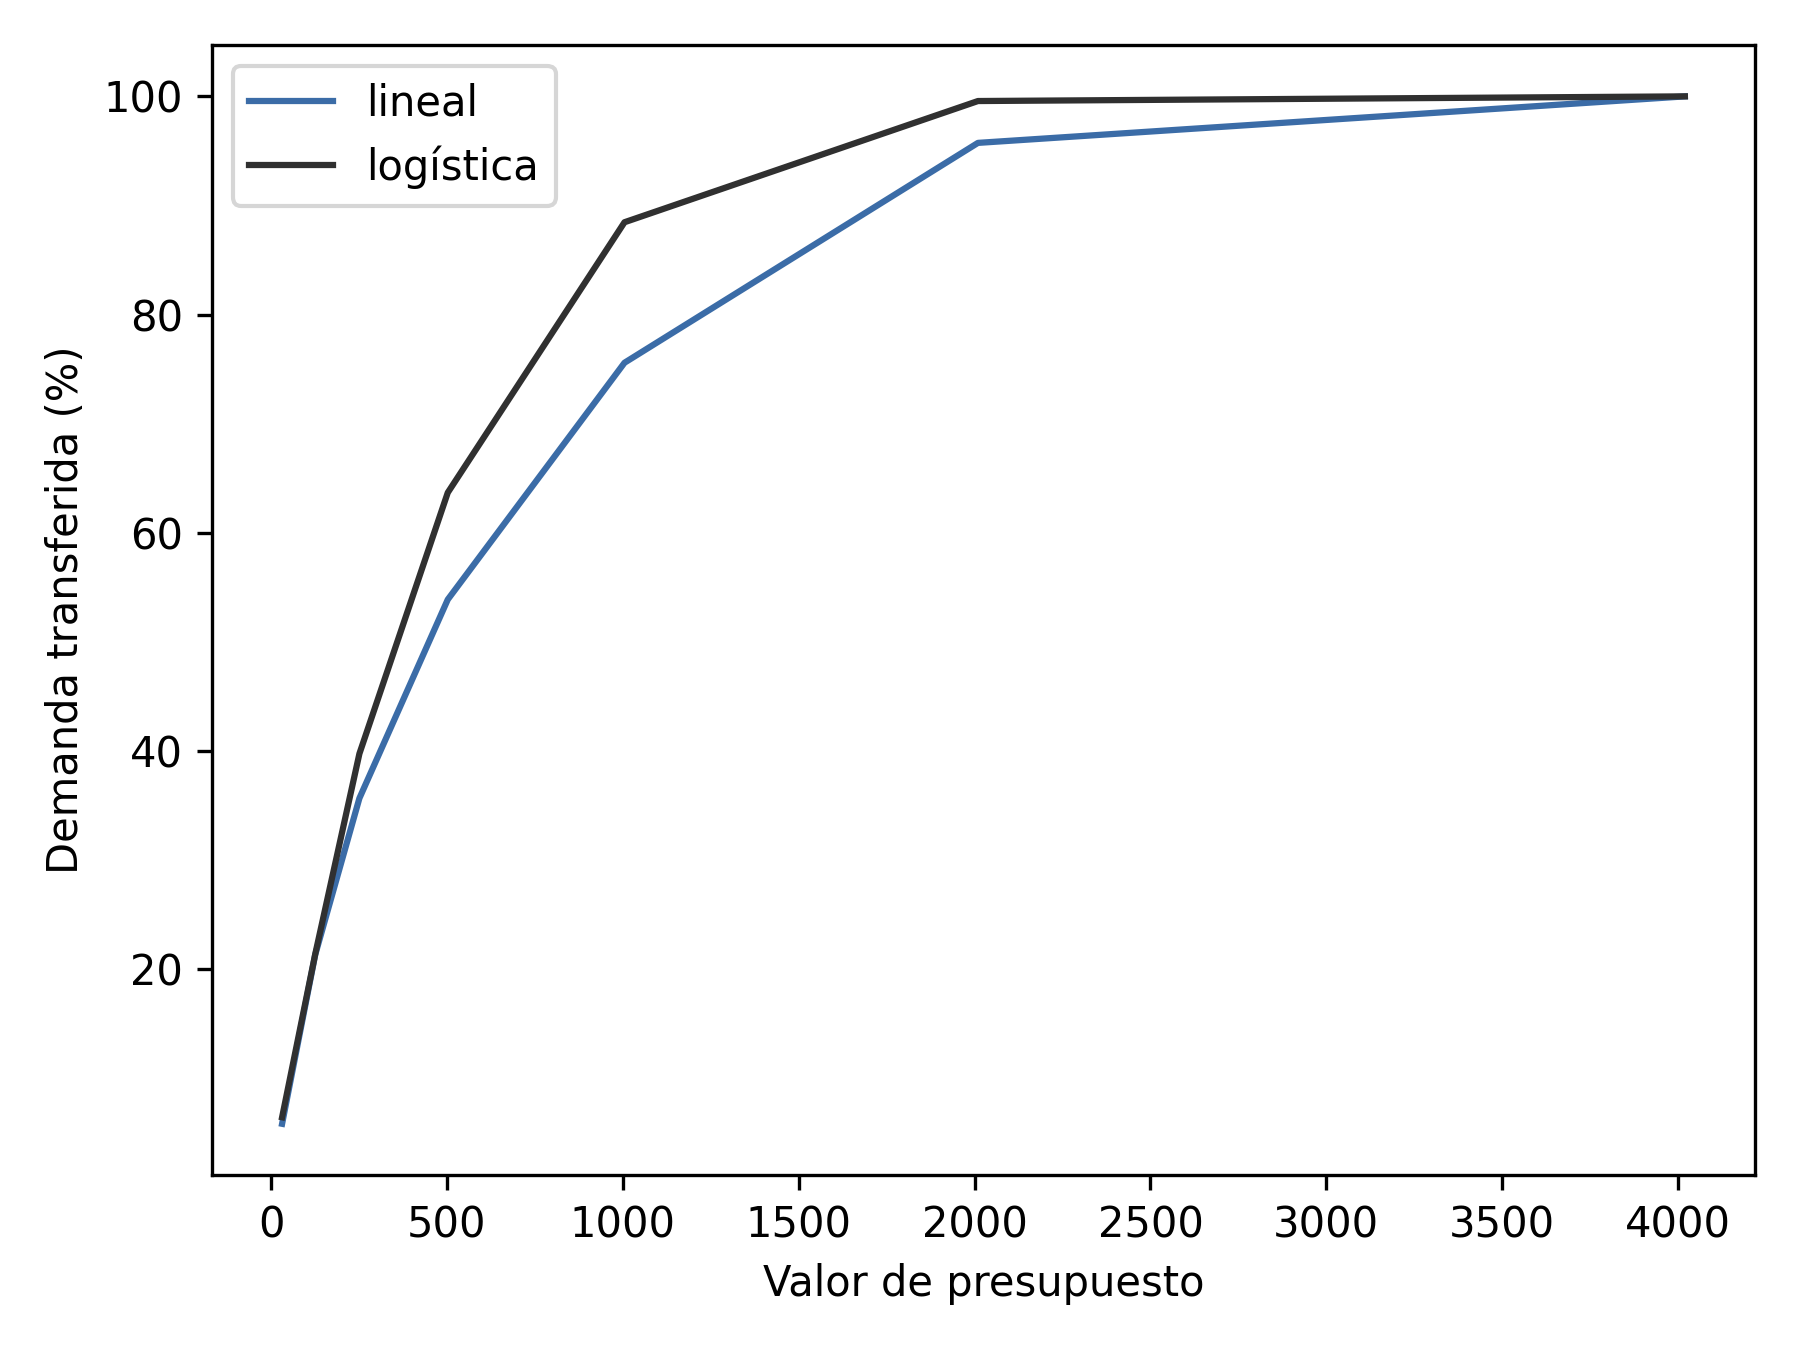
\includegraphics[width=8cm]{../resources/demand_by_budget.png}
    \caption{Porcentaje de demanda transferida total en función del presupuesto asignado para Sioux-Falls utilizando 20 puntos de quiebre y las funciones de transferencia de demanda lineal y logística. El comportamiento es similar en ambos casos y muestra que la eficiencia de aumentar el presupuesto no es siempre la misma.}
  \label{fig:demandtransferbybudgetlinear}
\end{figure}

Respecto a la utilización del presupuesto, vemos que a mayor presupuesto mayor es el porcentaje de gasto en los tipos de tecnologías más caras, lo cual es esperable dado que benefician más al usuario. Por otro lado, aumentar la cantidad de puntos de quiebre manteniendo presupuesto y función de transferencia fijas hace que el gasto en los tipos de tecnologías varíe, no necesariamente concentrando el gasto en los tipos más caros. El desglose del presupuesto utilizado por tecnología se detalla en la Tabla \ref{table:sensibilitybudgetusage} y en la Figura \ref{fig:sensibilitybudgetusage}.

Respecto a la complejidad de cada instancia y su relación con el tiempo de ejecución debemos notar que si bien hacemos referencia a esta relación en base a los resultados, entendemos que para sacar conclusiones al respecto deberíamos realizar un buen número de ejecuciones para cada instancia en lo que en CPLEX se llama modo oportunista, es decir paralelizar al máximo sin garantizar determinismo.

\begin{sidewaystable}
  \centering
  \small
  \begin{tabular}{cccccc}
      \toprule
      Instancia & Factor de presupuesto & \shortstack{Cantidad de puntos \\ de quiebre} & \shortstack{Función de \\ transferencia} & Demanda transferida (\%) & \shortstack{Tiempo ejecución \\ (hh:mm:ss)} \\
      \midrule
      1 & 0,1 & 5 & lineal & 4,65 & 00:00:02 \\
      2 & 0,1 & 20 & lineal & 5,81 & 00:00:11 \\
      3 & 0,1 & 5 & logística & 5,13 & 00:00:01 \\
      4 & 0,1 & 20 & logística & 6,41 & 00:00:08 \\
      5 & 0,4 & 5 & concavidad negativa & 32,43 & 00:00:36 \\
      6 & 0,4 & 20 & concavidad negativa & 36,49 & 00:07:40 \\
      7 & 0,4 & 50 & concavidad negativa & 37,39 & 00:07:29 \\
      8 & 0,4 & 5 & concavidad positiva & 15,50 & 00:00:18 \\
      9 & 0,4 & 20 & concavidad positiva & 17,05 & 00:09:38 \\
      10 & 0,4 & 50 & concavidad positiva & 18,22 & 14:07:09 \\
      11 & 0,4 & 5 & lineal & 18,60 & 00:00:24 \\
      12 & 0,4 & 20 & lineal & 21,32 & 00:06:17 \\
      13 & 0,4 & 50 & lineal & 22,09 & 00:31:55 \\
      14 & 0,4 & 5 & logística & 18,80 & 00:00:27 \\
      15 & 0,4 & 20 & logística & 21,37 & 00:12:35 \\
      16 & 0,4 & 50 & logística & 23,08 & 00:43:53 \\
      17 & 0,8 & 5 & lineal & 32,17 & 00:00:59 \\
      18 & 0,8 & 20 & lineal & 35,66 & 01:26:32 \\
      19 & 0,8 & 5 & logística & 35,47 & 00:00:44 \\
      20 & 0,8 & 20 & logística & 39,74 & 00:05:20 \\
      21 & 1,6 & 5 & lineal & 49,22 & 00:03:22 \\
      22 & 1,6 & 20 & lineal & 53,88 & 00:55:20 \\
      23 & 1,6 & 5 & logística & 58,97 & 00:02:36 \\
      24 & 1,6 & 20 & logística & 63,68 & 00:35:05 \\
      25 & 3,2 & 5 & lineal & 71,71 & 00:00:54 \\
      26 & 3,2 & 20 & lineal & 75,58 & 00:07:49 \\
      27 & 3,2 & 5 & logística & 80,77 & 00:01:33 \\
      28 & 3,2 & 20 & logística & 88,46 & 00:02:39 \\
      29 & 6,4 & 5 & lineal & 94,57 & 00:00:05 \\
      30 & 6,4 & 20 & lineal & 95,74 & 00:00:22 \\
      31 & 6,4 & 5 & logística & 97,44 & 00:00:02 \\
      32 & 6,4 & 20 & logística & 99,57 & 00:00:01 \\
      33 & 12,8 & 5 & lineal & 100,00 & 00:00:00 \\
      34 & 12,8 & 20 & lineal & 100,00 & 00:00:00 \\
      35 & 12,8 & 5 & logística & 100,00 & 00:00:00 \\
      36 & 12,8 & 20 & logística & 100,00 & 00:00:00 \\
      \bottomrule
  \end{tabular}
  \caption{Todas las instancias fueron solucionadas al óptimo en tiempos relativamente cortos, con excepción de dos instancias cuyo tiempo de ejecución fue más de una hora.} \label{table:sensibilityresults}
\end{sidewaystable}

\begin{sidewaystable}
  \centering
  \small
  \begin{tabular}{cccccccc}
      \toprule
      Instancia & Presupuesto & Presupuesto utilizado & Tecn. 1 (\%) & Tecn. 2 (\%) & Tecn. 3 (\%) & Tecn. 4 (\%) & Tecn. 5 (\%) \\
      \midrule
      1 & 31.4 & 31 & 35.48 & 64.52 &  &  &  \\
      2 & 31.4 & 31 & 9.68 & 90.32 &  &  &  \\
      3 & 31.4 & 30 &  & 46.67 & 53.33 &  &  \\
      4 & 31.4 & 31 & 9.68 & 51.61 & 38.71 &  &  \\
      5 & 125.6 & 125 & 10.4 & 83.2 & 6.4 &  &  \\
      6 & 125.6 & 125 & 4.0 & 89.6 & 6.4 &  &  \\
      7 & 125.6 & 125 & 5.6 & 81.6 & 12.8 &  &  \\
      8 & 125.6 & 125 & 2.4 & 24.0 & 41.6 & 32.0 &  \\
      9 & 125.6 & 125 & 7.2 & 12.8 & 48.0 & 32.0 &  \\
      10 & 125.6 & 125 & 2.4 & 27.2 & 51.2 & 19.2 &  \\
      11 & 125.6 & 125 & 15.2 & 33.6 & 51.2 &  &  \\
      12 & 125.6 & 125 & 16.8 & 70.4 & 12.8 &  &  \\
      13 & 125.6 & 125 & 5.6 & 81.6 & 12.8 &  &  \\
      14 & 125.6 & 125 & 4.0 & 44.8 & 38.4 & 12.8 &  \\
      15 & 125.6 & 125 & 5.6 & 11.2 & 70.4 & 12.8 &  \\
      16 & 125.6 & 125 & 2.4 & 36.8 & 60.8 &  &  \\
      17 & 251.2 & 251 & 5.18 & 35.86 & 36.65 & 22.31 &  \\
      18 & 251.2 & 251 & 8.37 & 21.51 & 70.12 &  &  \\
      19 & 251.2 & 251 & 1.99 & 21.51 & 44.62 & 31.87 &  \\
      20 & 251.2 & 251 & 1.2 & 11.16 & 81.27 & 6.37 &  \\
      21 & 502.4 & 502 & 0.4 & 15.94 & 19.92 & 63.75 &  \\
      22 & 502.4 & 502 & 2.39 & 7.57 & 45.42 & 44.62 &  \\
      23 & 502.4 & 501 & 2.2 & 13.97 & 35.93 & 47.9 &  \\
      24 & 502.4 & 502 & 2.79 & 5.58 & 54.98 & 36.65 &  \\
      25 & 1004.8 & 1002 & 0.4 & 4.19 & 13.17 & 19.96 & 62.28 \\
      26 & 1004.8 & 1004 &  & 5.98 & 6.37 & 49.4 & 38.25 \\
      27 & 1004.8 & 1004 & 0.6 & 2.99 & 26.29 & 17.53 & 52.59 \\
      28 & 1004.8 & 1004 & 0.8 & 1.2 & 14.34 & 83.67 &  \\
      29 & 2009.6 & 2008 &  & 0.4 & 4.38 & 3.59 & 91.63 \\
      30 & 2009.6 & 2008 &  & 0.4 & 1.59 & 10.36 & 87.65 \\
      31 & 2009.6 & 2008 & 0.1 & 1.49 & 2.39 & 1.99 & 94.02 \\
      32 & 2009.6 & 2004 &  & 0.6 & 1.6 & 14.77 & 83.03 \\
      33 & 4019.2 & 2719 & 0.26 & 0.29 & 1.18 &  & 98.27 \\
      34 & 4019.2 & 3048 &  & 0.26 &  &  & 99.74 \\
      35 & 4019.2 & 2780 & 0.14 & 0.86 &  &  & 98.99 \\
      36 & 4019.2 & 2994 & 0.07 &  & 0.53 &  & 99.4 \\
      \bottomrule
  \end{tabular}
  \caption{Detalle de presupuesto utilizado por instancia por tipo de tecnología. Las columnas Presupuesto y Presupuesto Utilizado están en unidades de presupuesto. Los porcentajes se calcularon sobre el valor de presupuesto utilizado y pueden no sumar 100\% por el redondeo realizado.} \label{table:sensibilitybudgetusage}
\end{sidewaystable}

\begin{figure}[h!]
  \centering
  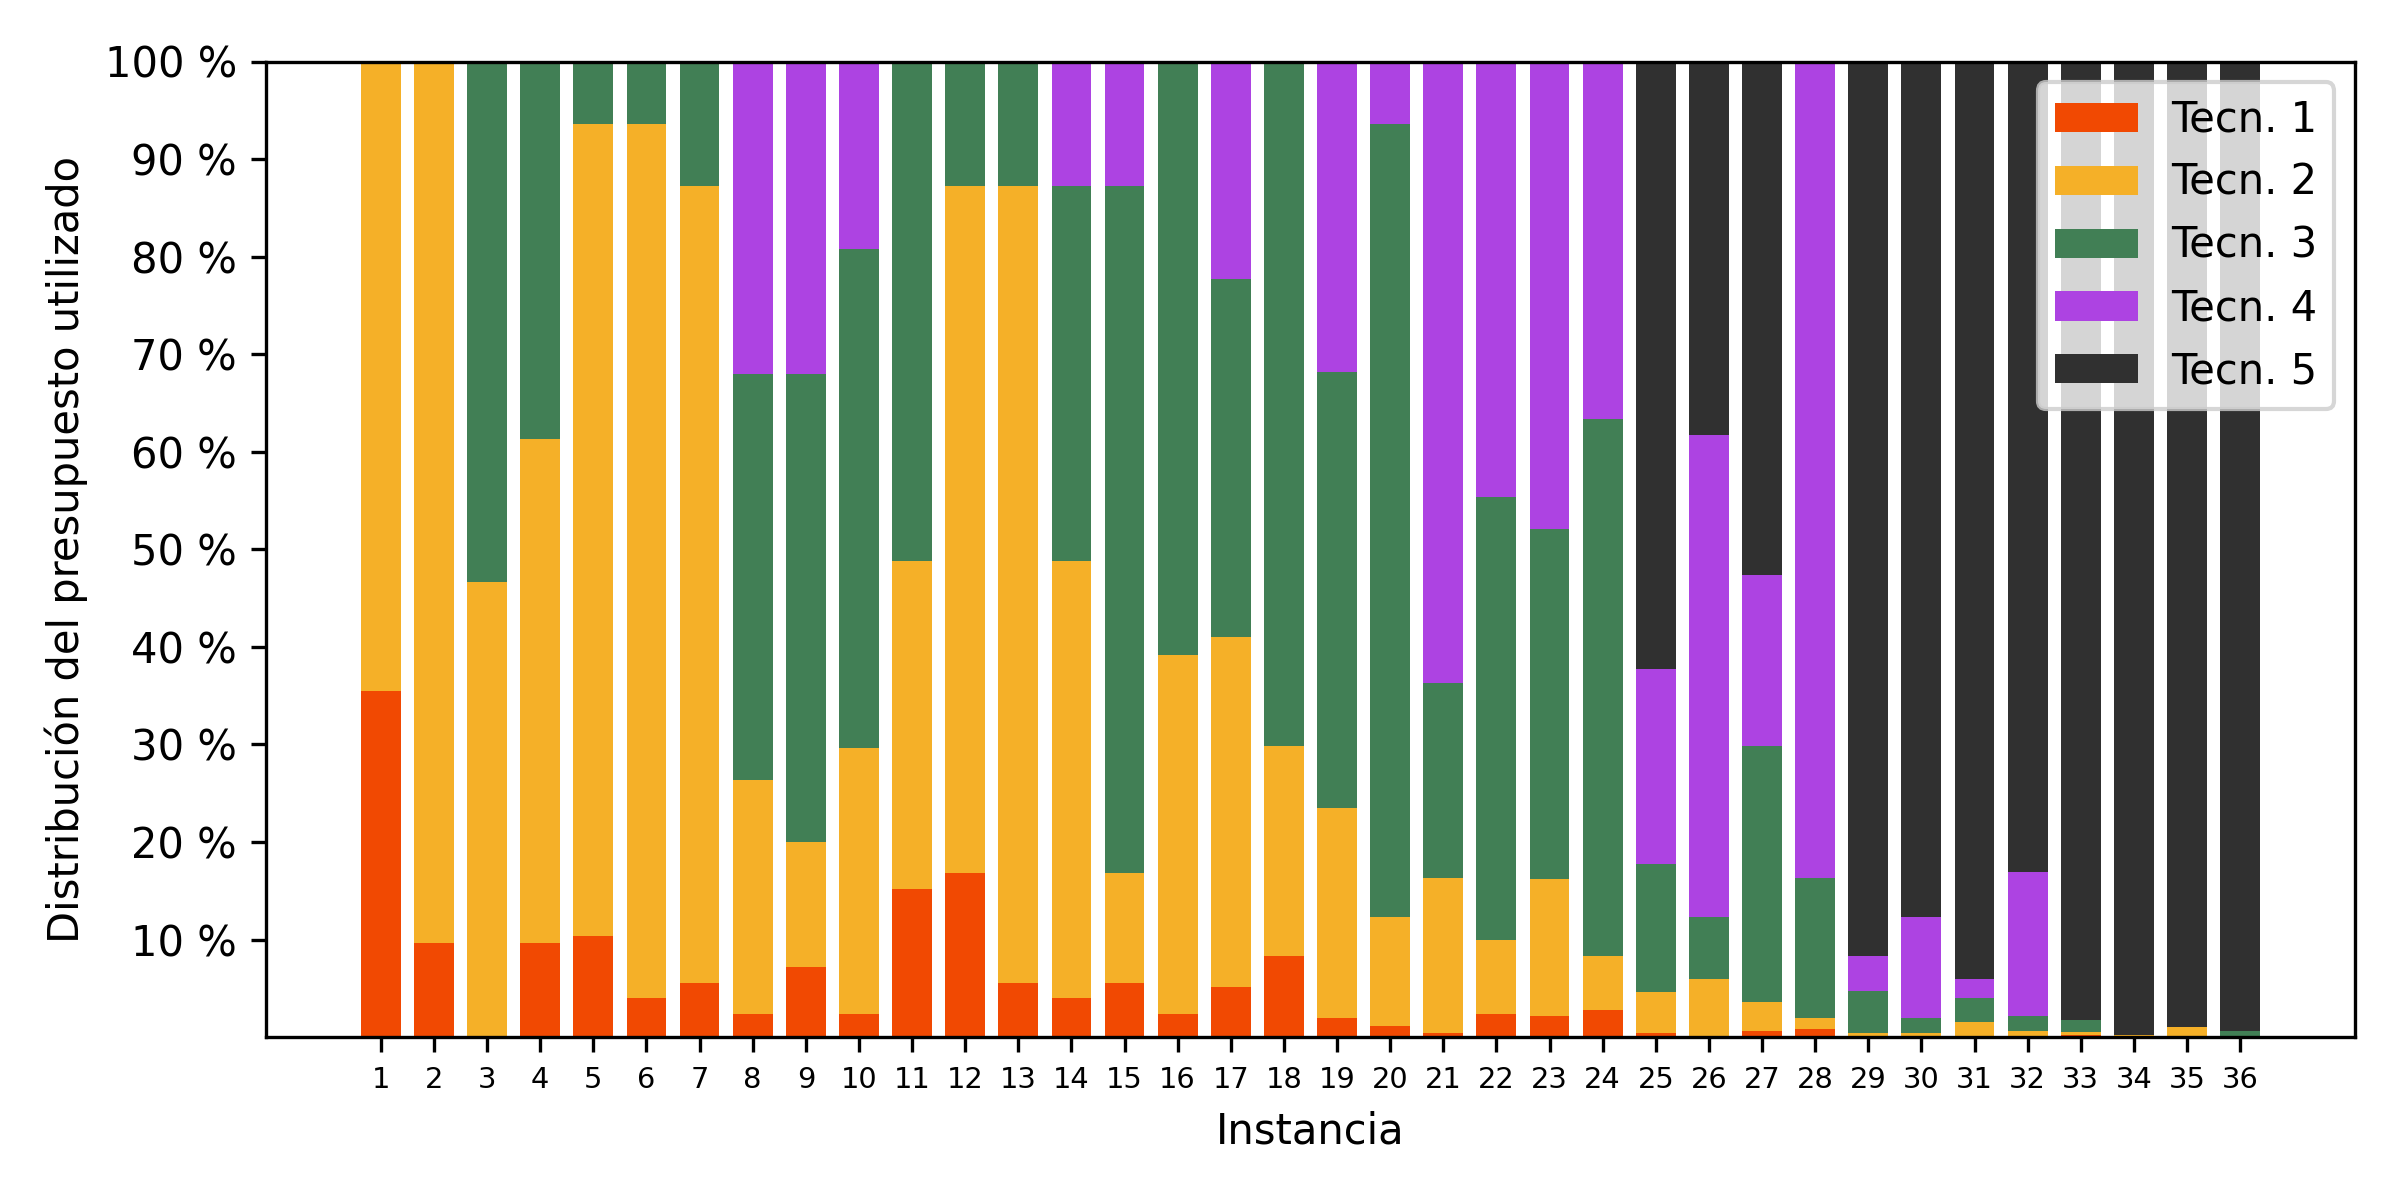
\includegraphics[width=14cm]{../resources/budget_use_by_infra.png}
  \caption{Visualización de la distribución del uso del presupuesto para cada instancia.}
  \label{fig:sensibilitybudgetusage}
\end{figure}

\begin{figure}[h!]
  \centering
  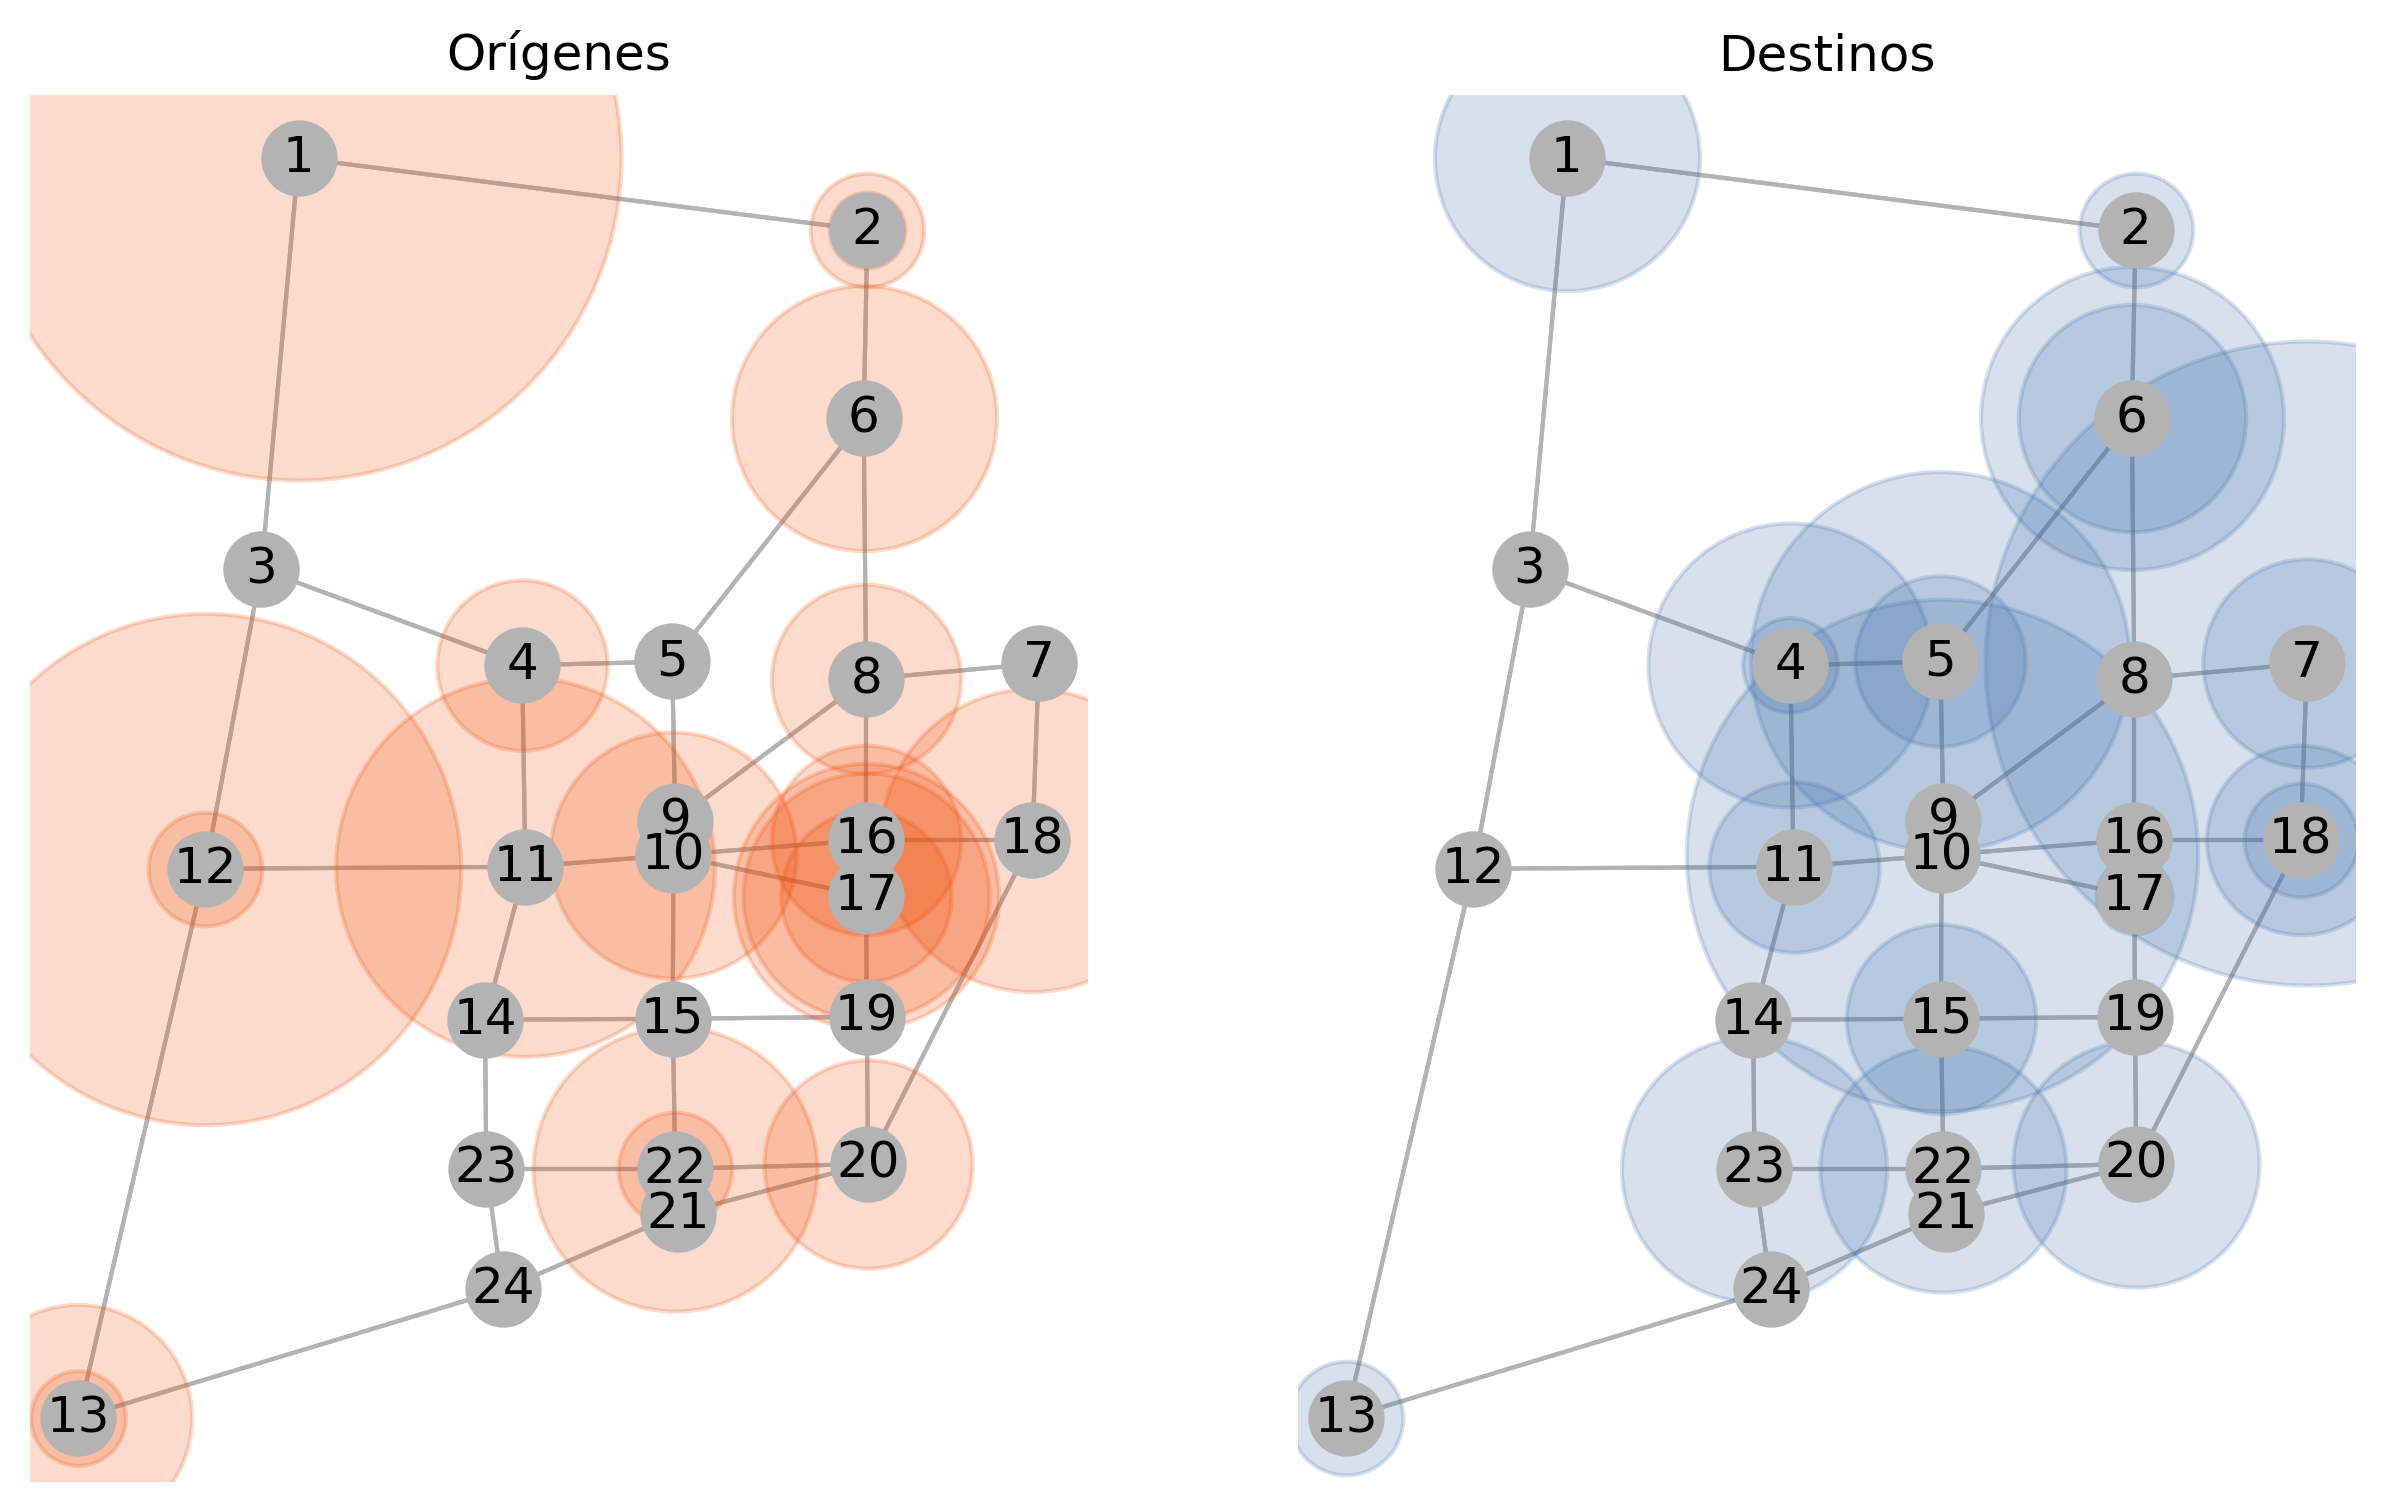
\includegraphics[width=12cm]{../resources/sioux_falls_demand.png}
  \caption{Visualización de la distribución de nodos origen y destino junto a su valor de demanda representado por el tamaño de los círculos para la instancia de Sioux-Falls. A la izquierda se ubican los orígenes y a la derecha los destinos. Los tamaños de los círculos son proporcionales al valor de demanda y no se suman por nodo.}
  \label{fig:sioux_falls_demand}
\end{figure}

\clearpage
\subsection*{Casos particulares}

Vamos a analizar en detalle algunos casos particulares y discutir cómo afecta la cantidad de puntos de quiebre a la decisiones de cuales tecnologías construir. Comparamos las instancias 11, 12 y 13, que utilizan la función lineal de transferencia de demanda con 5, 20 y 50 puntos de quiebre respectivamente y un factor de presupuesto de 40\%. Más datos específicos de cada instancia se pueden apreciar en la Tabla \ref{table:sensibilityinfralengths} y Figura \ref{fig:sensibilityinstance11_12_13}. Observamos que a mayor cantidad de puntos de quiebre más inteligentes son las decisiones tomadas. Por ejemplo, en la instancia 11 la mitad del acotado presupuesto se invirtió en poco cubrimiento de calles utilizando la tecnología 3 mientras que en la 12 y 13 el gasto en esta tecnología sólo fue el 12\%. En las instancias 12 y 13 la mayor parte del gasto se hizo en tecnología 2 que para el nivel de presupuesto y función de transferencia de demanda parece ser la más eficiente. En particular, los datos de porcentaje del largo total de las calles cubierto desglosado por tipo de tecnología nos da una idea general de la demanda afectada, al ser esta instancia altamente densa y uniforme en términos de orígenes y destinos, como se observa en la Figura \ref{fig:sioux_falls_demand}.

 \begin{table}[h!]
  \centering
  \begin{tabular}{ccccc}
    \toprule
      Instancia & Tecn. 1 (\%) & Tecn. 2 (\%) & Tecn. 3 (\%) & Total (\%) \\
    \midrule
      11 & 8,74  & 6,51   & 5,72 & 20,98 \\
      12 & 8,89  & 15,22  & 1,64 & 25,75 \\
      13 & 2,29  & 17,77  & 1,96 & 22,73 \\
    \bottomrule
  \end{tabular}
  \caption{Porcentaje del largo total de arcos de la red construido con cada tipo de tecnología (excluyendo la tecnología base) para las instancias de interés.}\label{table:sensibilityinfralengths}
\end{table}

Si observamos los datos de demanda transferida y costo de camino más corto, Figura \ref{fig:sensibilitybyodpair_11_12_13}, vemos que a mayor cantidad de puntos de quiebre mayor es la cantidad de pares origen-destino afectada aunque en general las decisiones de cuáles pares origen-destino y cuánto mejorarlos no fue muy diferente entre instancias.

\begin{figure}[h!]
  \centering
  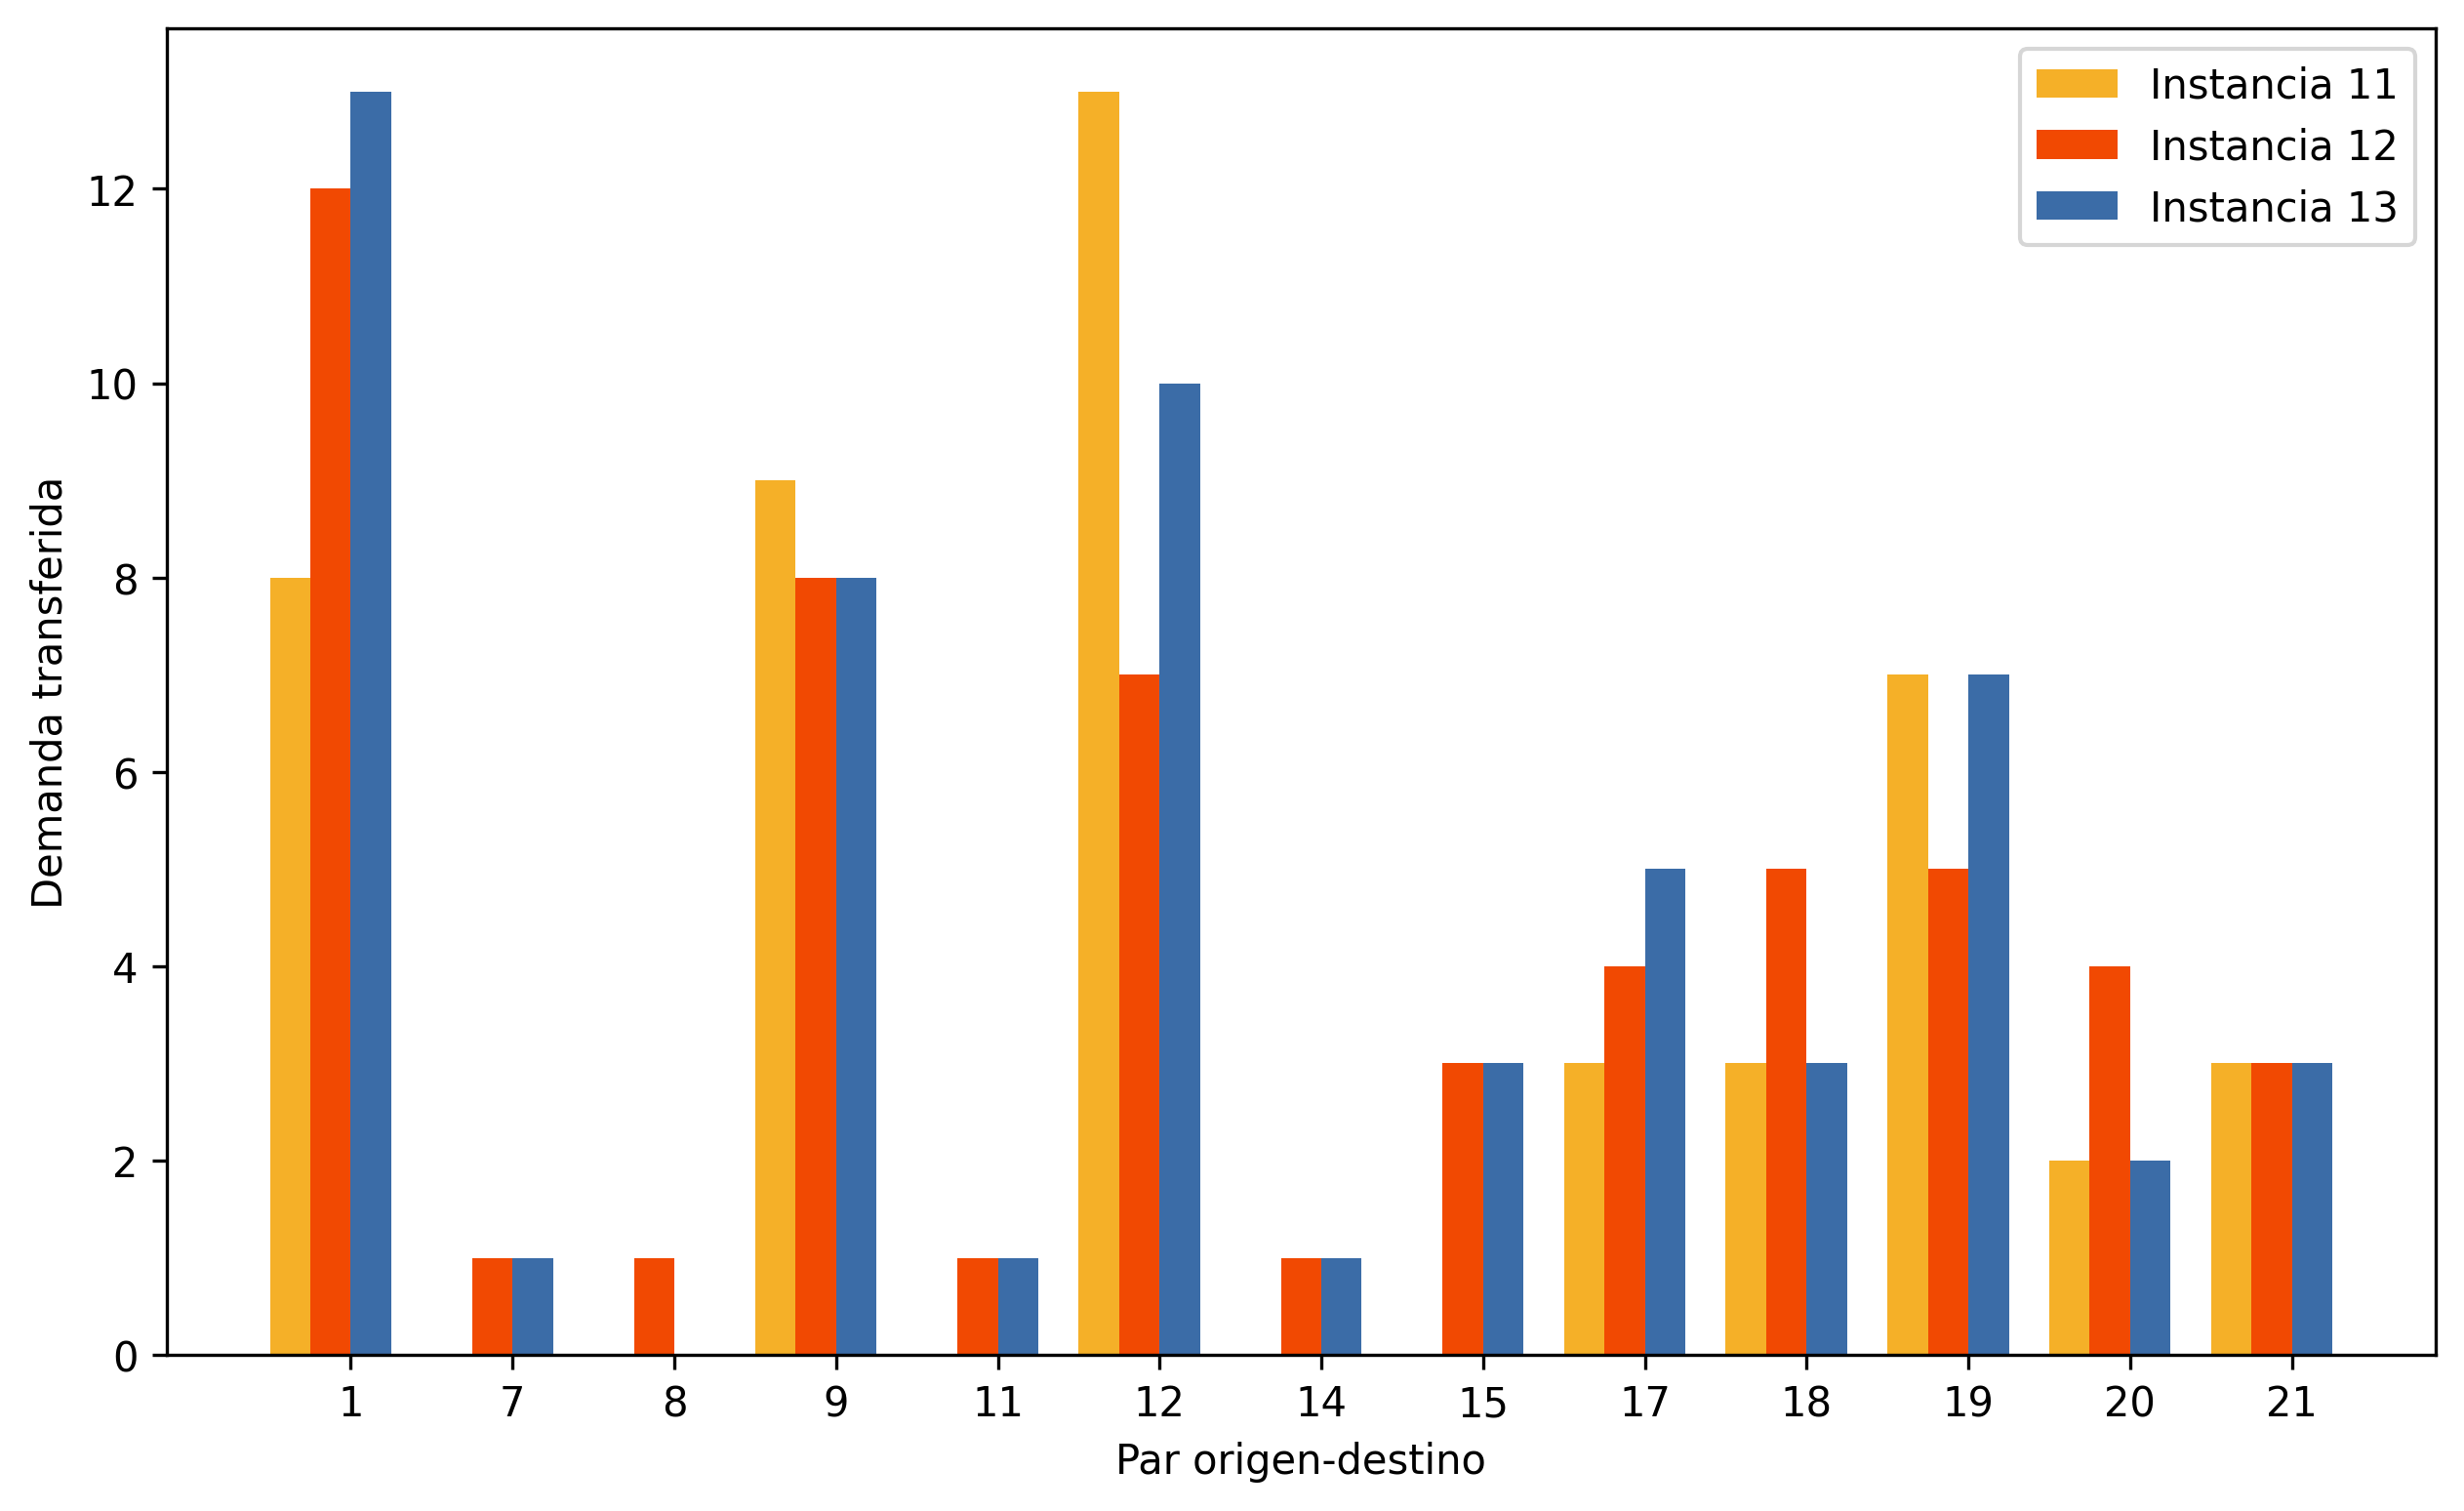
\includegraphics[width=12cm]{../resources/sensibility_case_study_demand.png}
  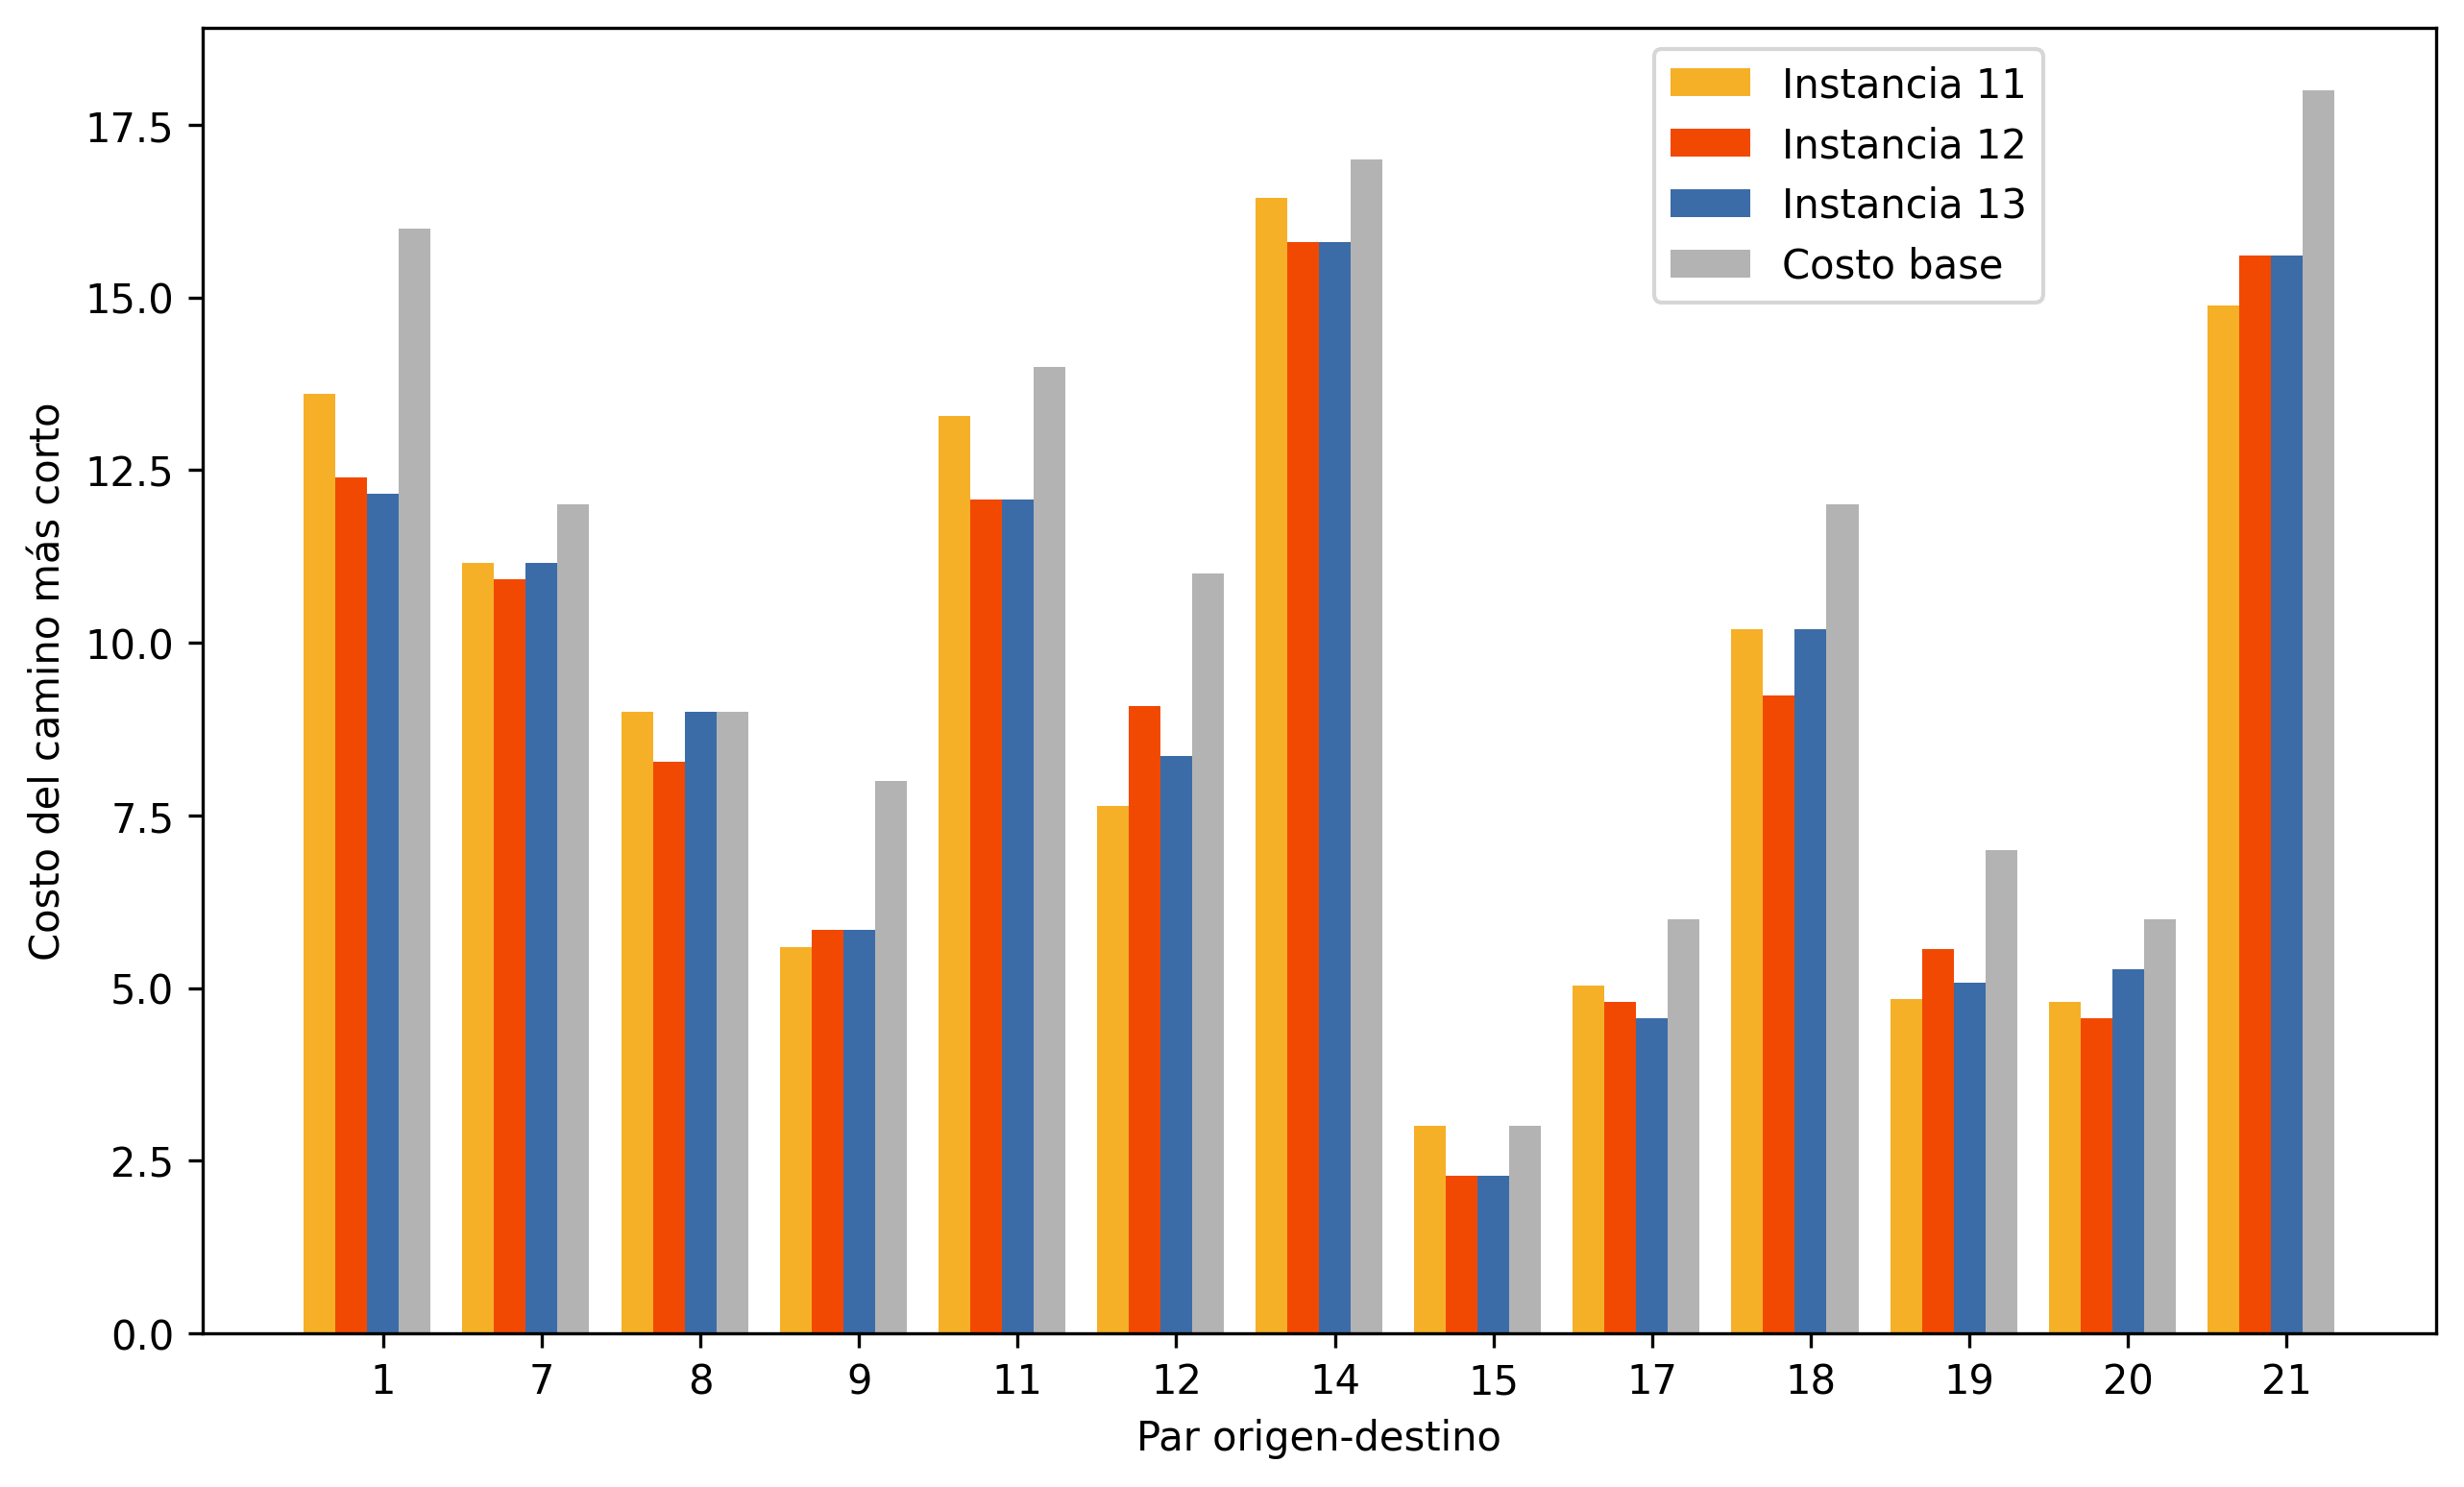
\includegraphics[width=12cm]{../resources/sensibility_case_study_shortest_paths.png}
  \caption{Demanda transferida y costo del camino más corto para los pares origen-destino para los cuales hubo demanda transferida. Los pares origen-destino se numeran de acuerdo a la Tabla \ref{table:siouxfallsdemanddata} en el Apéndice \ref{sect:siouxfallsdata}. Los costos de los caminos más cortos se comparan contra el costo base que es aquel sobre la red en la cual no hay infraestructura de ciclovía construida.}
  \label{fig:sensibilitybyodpair_11_12_13}
\end{figure}

\begin{figure}[h!]
  \centering
  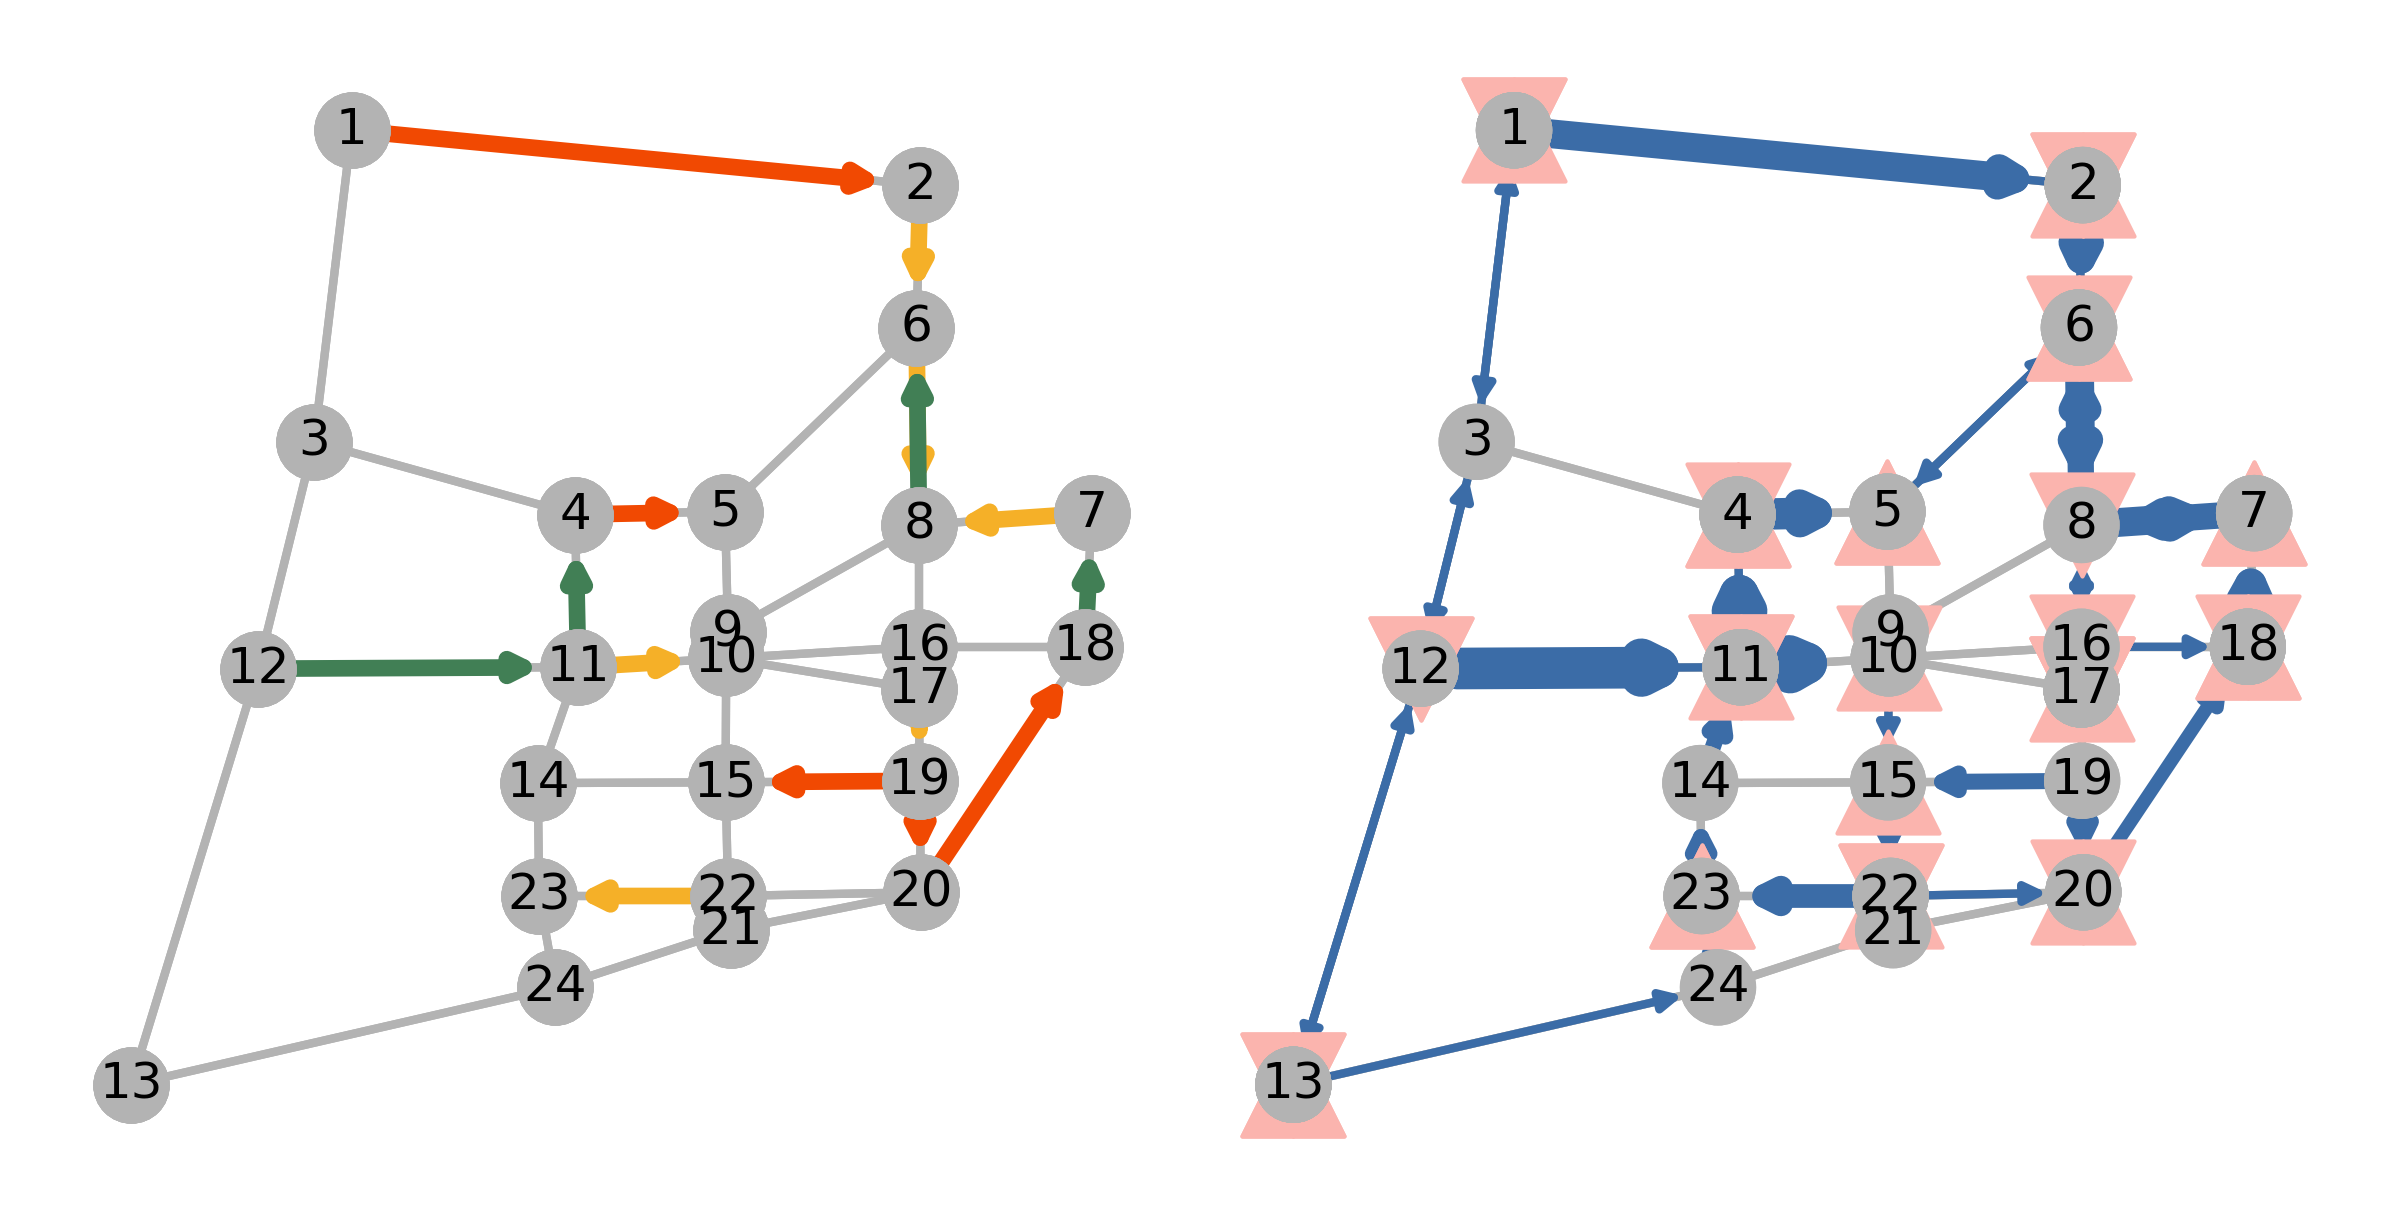
\includegraphics[width=10cm]{../resources/sioux_falls_0.4_budget_factor_linear_5_breakpoints.png}
  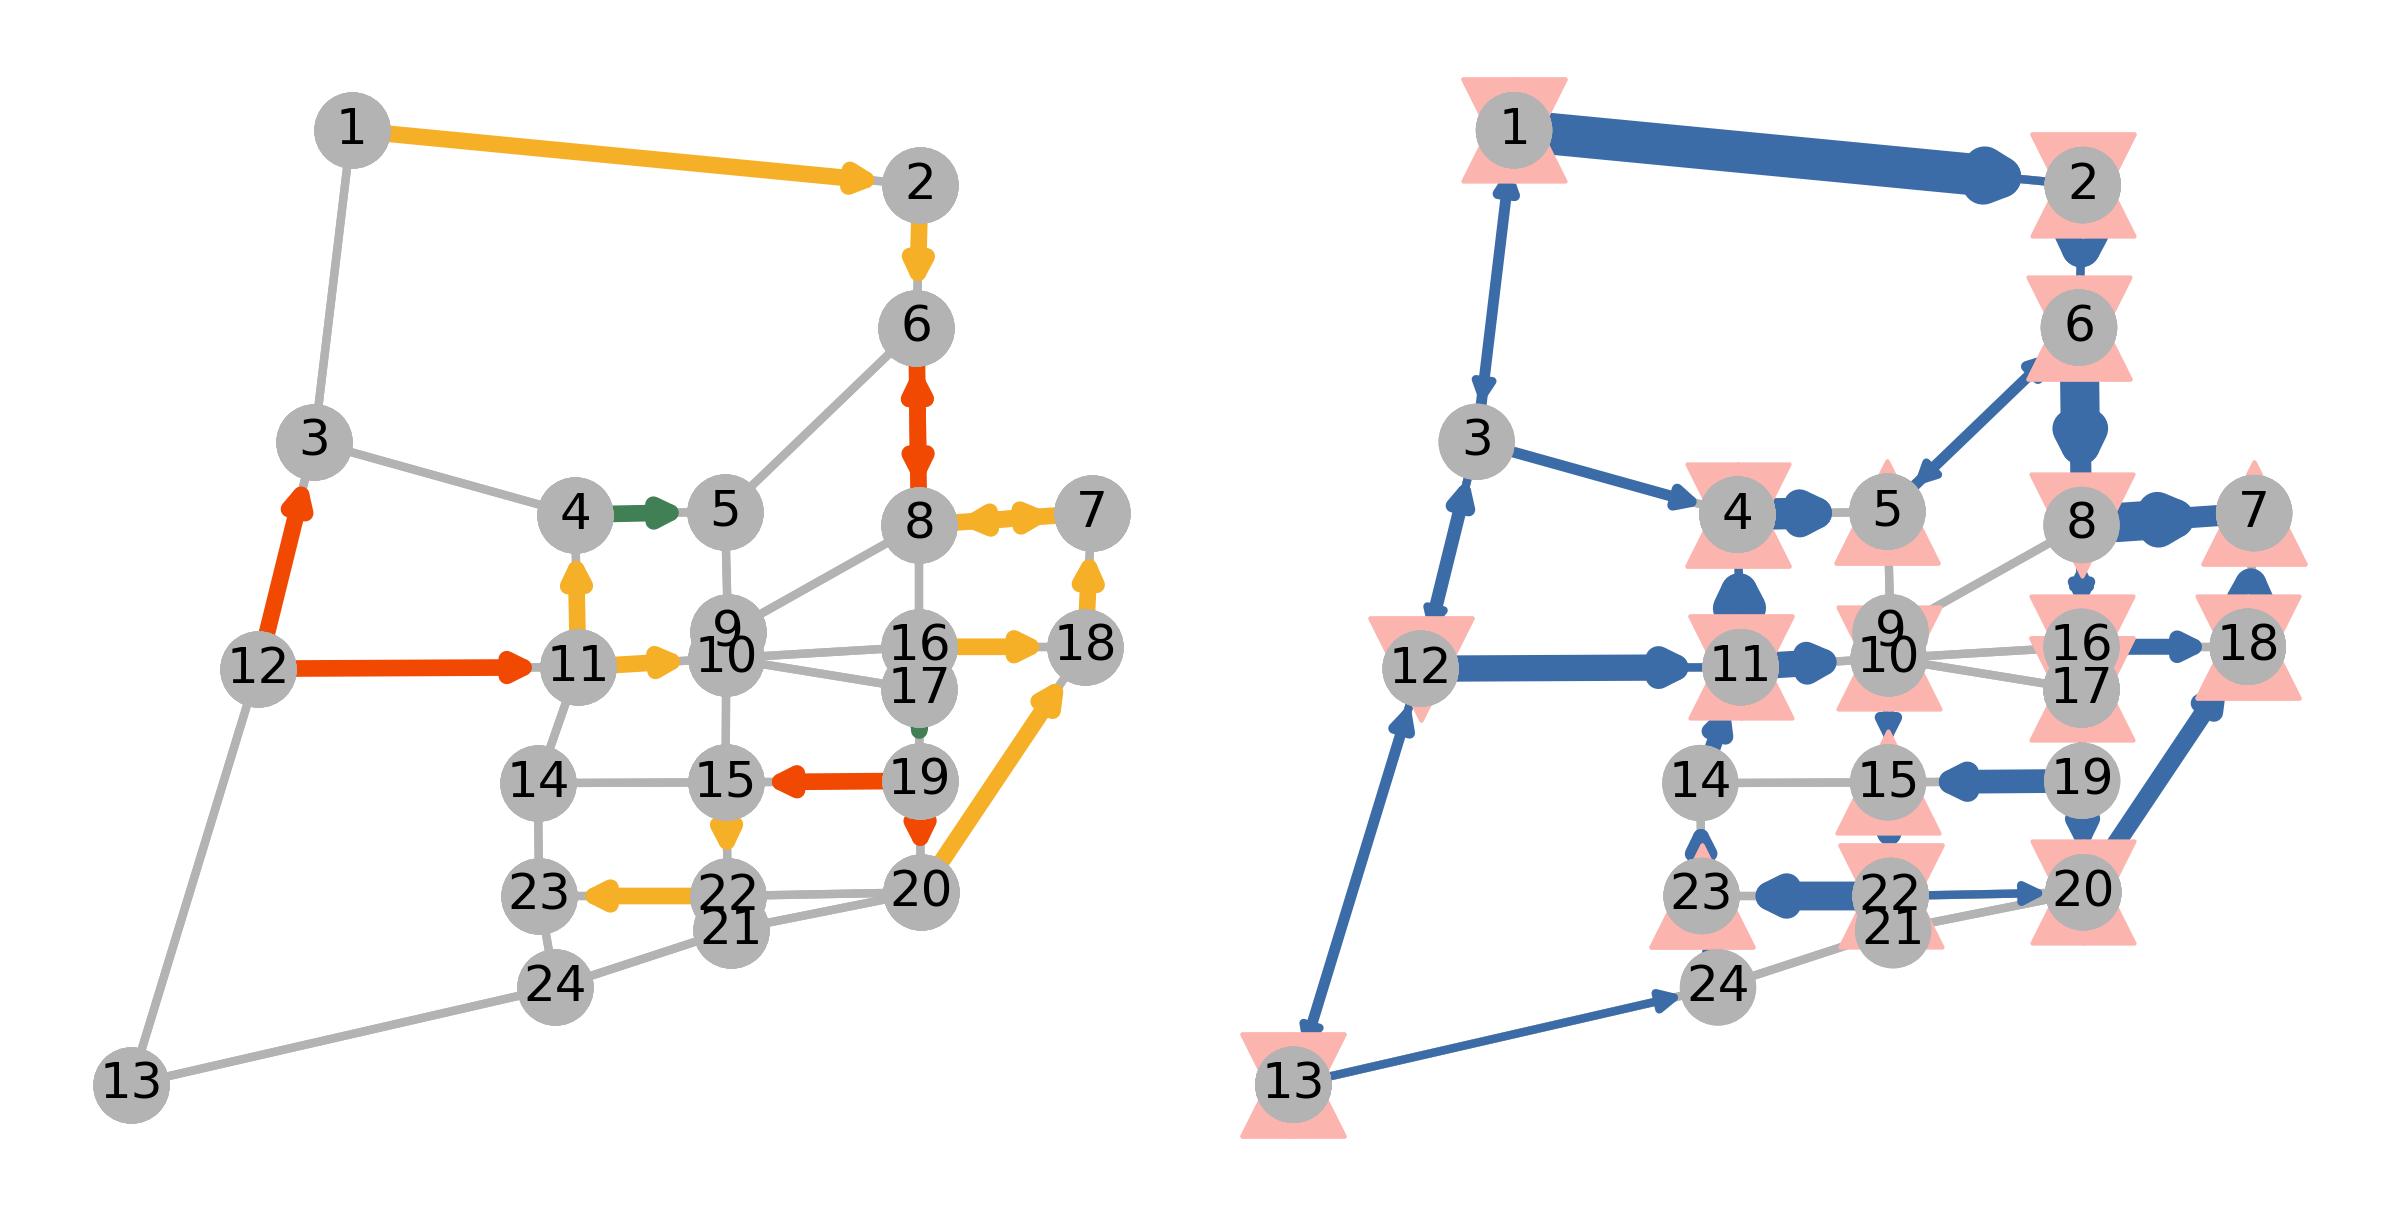
\includegraphics[width=10cm]{../resources/sioux_falls_0.4_budget_factor_linear_20_breakpoints.png}
  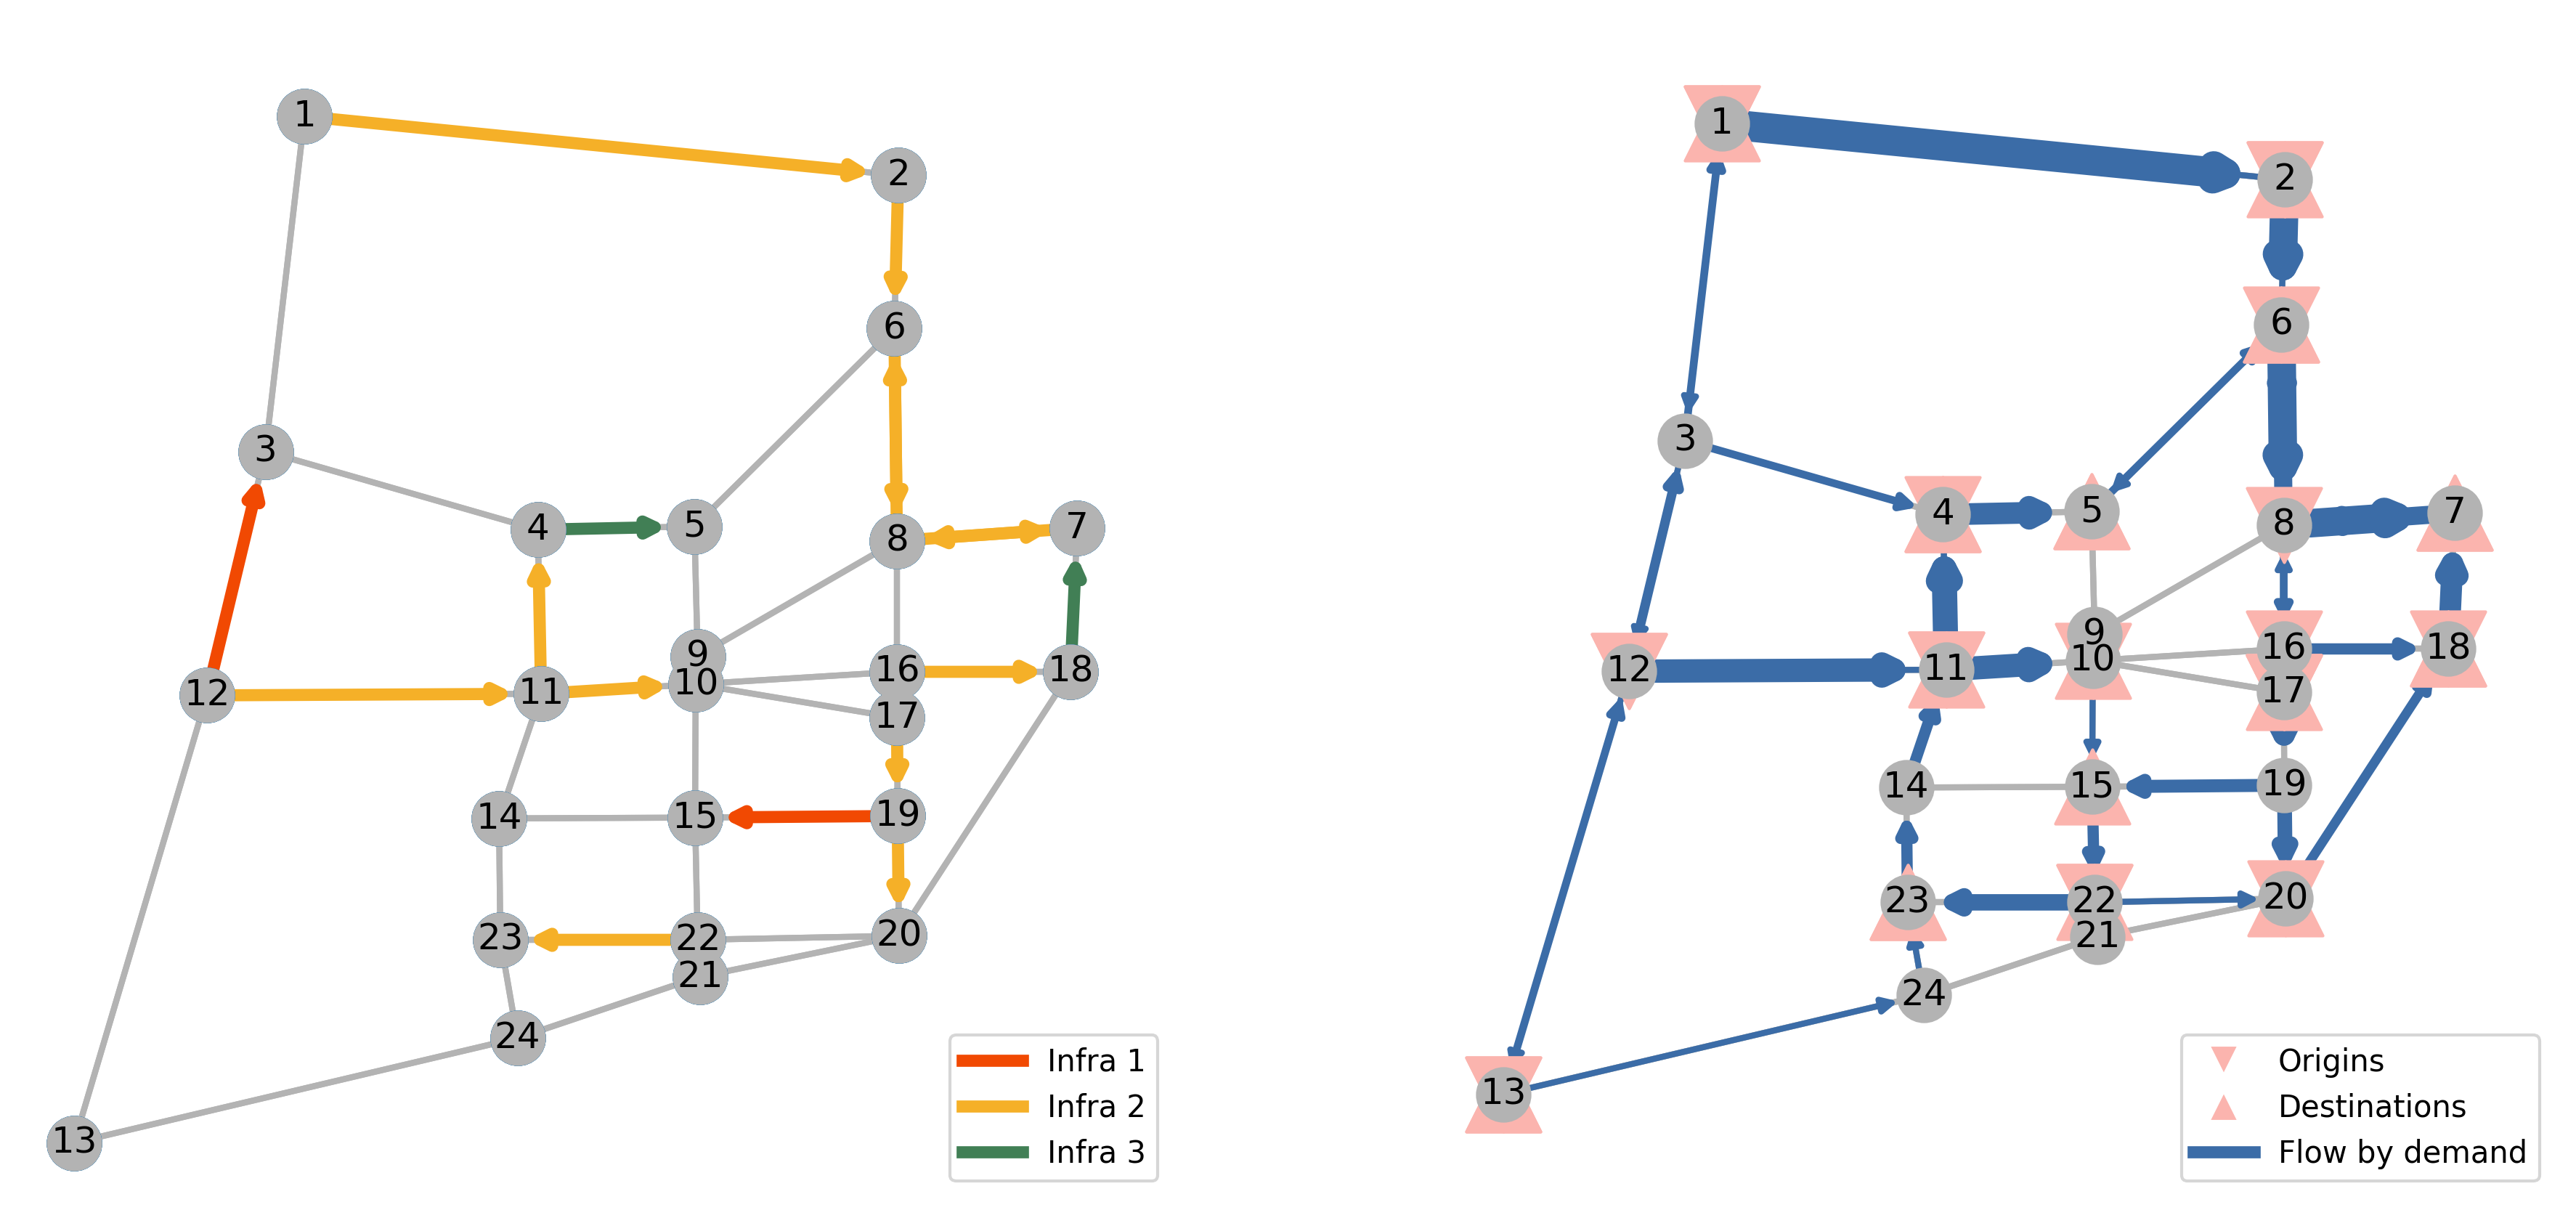
\includegraphics[width=10cm]{../resources/sioux_falls_0.4_budget_factor_linear_50_breakpoints.png}
  \caption{De arriba hacia abajo, instancia 11, 12 y 13. A la izquierda se muestran las ubicaciones de cada tipo de tecnología. A la derecha los flujos para cada arco considerando el acumulado de demanda de cada par origen-destino que pasaría sobre ellos. Los flujos no se agregan entre dos arcos adyacentes con sentido opuesto, en dicho caso solo se visualiza el mayor de los flujos.}
  \label{fig:sensibilityinstance11_12_13}
\end{figure}

\FloatBarrier
\section{Aplicación a un caso real}

Utilizamos una instancia de la ciudad de Montevideo de manera de poder analizar la aplicación práctica del problema sobre datos familiares y realistas. Los datos de la instancia provienen de una red sobre una zonificación de la ciudad que resulta en un grafo de 136 nodos y 636 arcos. Respecto a la demanda, consideramos los 600 pares origen-destino de mayor demanda que cumplen que el origen y destino no se encuentran a más de 3 km de distancia euclídea entre ellos. Encontramos que una distancia 3 km en línea recta, que implica una distancia Manhattan máxima de poco más de 4.2 km, es un límite razonable para viajes en bicicleta común y eléctricas según \cite{anette2018}, donde se estima una distancia de viaje promedio de 2.6 km y 3 km respectivamente. Además, está dentro de lo que \cite{shwe2014} considera un viaje potencial en bicicleta, es decir, menor a 5 km.

\subsection{Descripción de la instancia}

La ciudad de Montevideo es de mayor tamaño en el Uruguay. Incluyendo el área metropolitana cuenta con una población de cerca de 1.8 millones de personas y una densidad de población de 6726 habitantes por $km^2$. La ciudad cuenta con un sistema de transporte de autobuses que, junto al transporte privado automotor, abarcan la mayor parte de la demanda de viajes \cite{Mauttone2017a}.

La instancia utilizada corresponde a una simplifición de la red de calles de la ciudad, observar la comparación en la Figura \ref{fig:montevideosimplification}. La red simplificada fue desarrollada dentro de un proyecto de la Comisión Sectorial de Investigación Científica, CSIC \footnote{\url{https://www.csic.edu.uy/}}, y consiste en una zonificación de la ciudad donde los nodos corresponden a los centroides de cada zona y los arcos modelan la adyacencia entre zonas. Por otro lado, la matriz de demanda se tomó del \cite{Massobrio2020}, en donde se realiza un estudio y relevamiento de la demanda de viajes de la ciudad a partir de datos de uso del sistema transporte público de pasajeros en la ciudad de Montevideo. Si bien los datos de demandas no son específicos del transporte en bicicleta, los utilizamos por ser uno de los conjuntos de datos de viajes más complejos que hay disponibles.

\begin{figure}[h!]
  \centering
  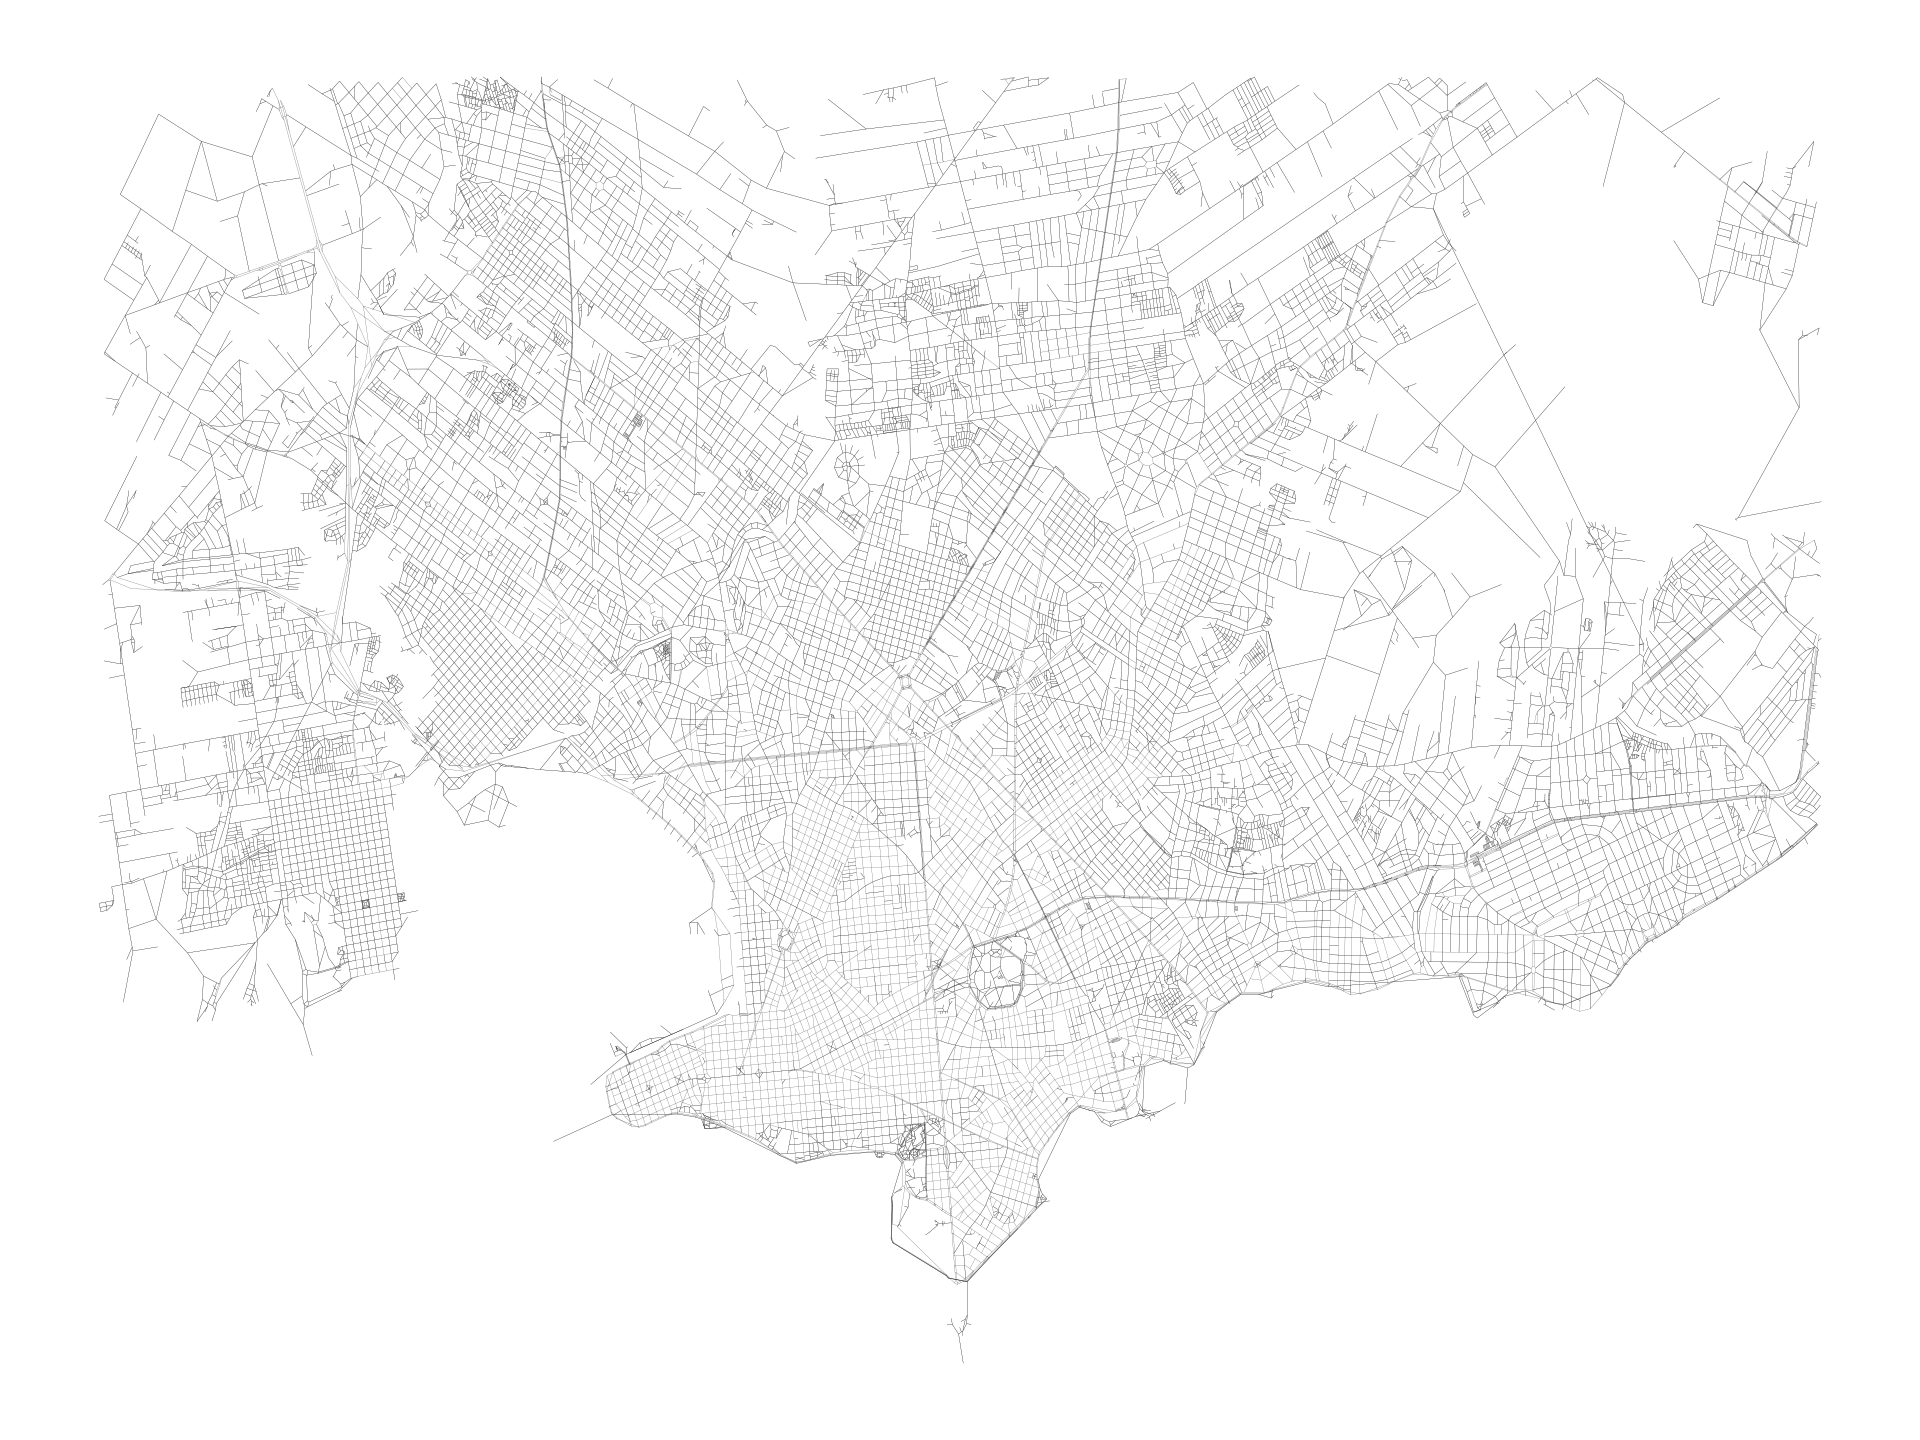
\includegraphics[width=10cm]{../resources/montevideo_full.png}
  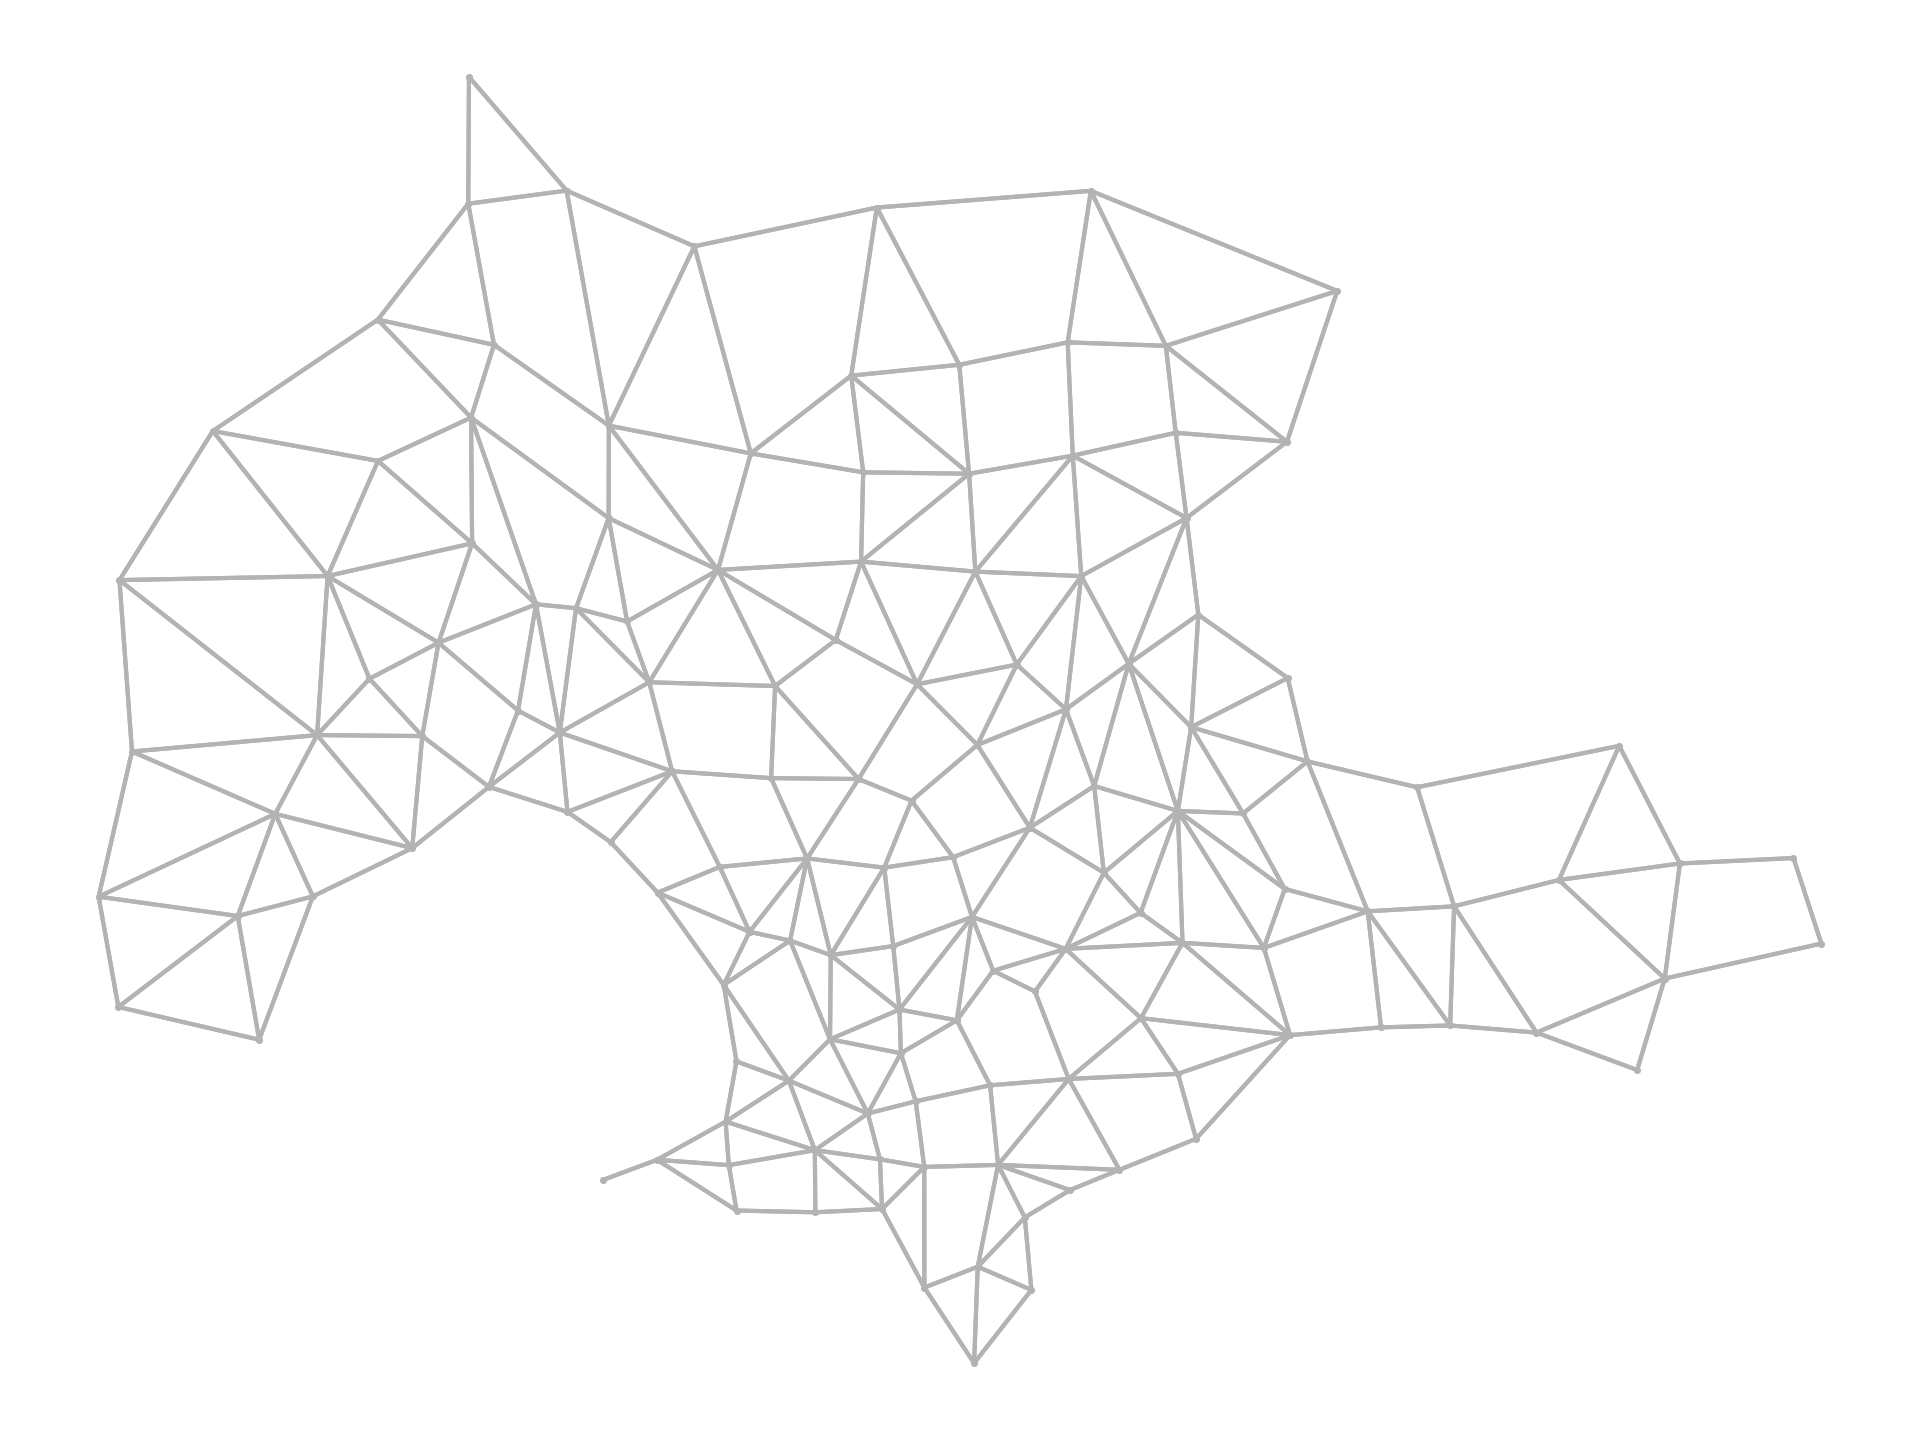
\includegraphics[width=10cm]{../resources/montevideo_simple.png}
  \caption{Compartiva de la red de calles de Montevideo y la red de la red utilizando la zonificación en 136 nodos y 636 arcos.}
  \label{fig:montevideosimplification}
\end{figure}

Actualmente la red de ciclovías en Montevideo abarca más de 48 km correspondiente a cerca de 1,27\% del largo total de la red de calles, ver Figura \ref{fig:montevideobikeways}. Se espera que esta red siga creciendo como parte de las políticas de incentivo del uso de la bicicleta que comprende 2,6\% del total viajes que se realizan \cite{Mauttone2017a}.

\begin{figure}[h!]
  \centering
  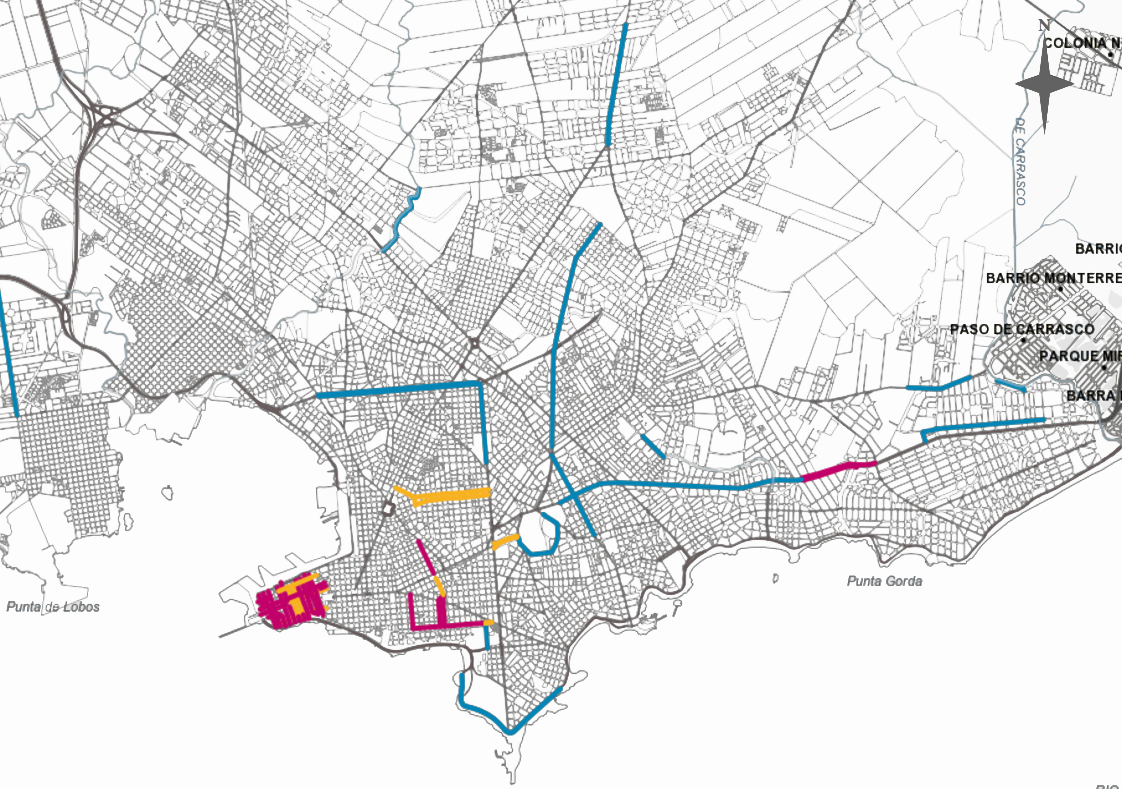
\includegraphics[width=10cm]{../resources/bicicircuitos_montevideo.png}
  \caption{Situación actual de la red de ciclovías en la ciudad de Montevideo. En color rojo se representa el tipo de tecnología más basico que en un límite de velocidad de 30 km/h para los vehiculos motorizados. En naranja la tecnología de nivel intermedio que a una senda específica para bicicletas dentro de la superficie de la calle. Por último, en azul, la tecnología superior correspondiente a una senda pavimentada exclusivamente construida para la bicicleta.}
  \label{fig:montevideobikeways}
\end{figure}

\subsection{Resultados}

Dado el tamaño de la instancia y los recursos computacionales disponibles decidimos utilizar 4 tipos de tecnología, incluyendo la base, y 10 puntos de quiebre. Probamos las funciones de transferencia de demanda logística y lineal y tres factores de presupuesto: 40\%, 80\% y 160\%. Las instancias fueron resueltas por el solver CPLEX versión 20.1.0.0, en un CPU Xeon Gold 6138 utilizando hasta 16 hilos y hasta 180 GB de memoria. CPLEX fue configurado para utilizar descomposición de Benders de manera automática, lo que nos permitió resolver de manera óptima las instancias estudiadas en unas pocas horas. Vale la pena mencionar que realizamos pruebas utilizando más tipos de tecnología y mayor cantidad de pares origen-destino pero nos encontramos con limitaciones en los recursos disponibles en términos de memoria o límite de tiempo de ejecución de 5 días.

El resumen de las ejecuciones se encuentra en la Tabla \ref{table:montevideoexecutions} y la asignación de presupuesto a cada tipo de tecnología de ciclovía en la Tabla \ref{table:montevideobudgetusage}. Observamos que los resultados son buenos en términos de demanda transferida para los casos con menor presupuesto en comparación con las instancias de Sioux-Falls. Podemos explicar esto porque la distribución de la proporción más significativa de la demanda en la red de Montevideo, como se puede ver en la Figura \ref{fig:montevideodemanddist}, se ubica en la misma región de la red. Por lo tanto concentrar la inversión en esa zona produce resultados de amplio impacto.

\begin{table}[h!]
  \centering
  \begin{adjustbox}{width=1.2\textwidth,center=\textwidth}
    \begin{tabular}{ccccccc}
      \toprule
        Instancia & \shortstack{Factor de \\ presupuesto} & \shortstack{Función de \\ transferencia} & \shortstack{\# Pares OD con \\ demanda transferida} & \shortstack{Demanda \\ transferida (\%)} & \shortstack{Tiempo de \\ ejecución \\ (hh:mm:ss)} \\
      \midrule
        1 & 0.4 & lineal & 395 & 53.92 & 02:59:57 \\
        2 & 0.4 & logística & 373 & 54.42 & 28:59:56 \\
        3 & 0.8 & lineal & 513 & 74.76 & 00:32:13 \\
        4 & 0.8 & logística & 510 & 75.76 & 00:37:32 \\
        5 & 1.6 & lineal & 598 & 94.7 & 00:14:26 \\
        6 & 1.6 & logística & 597 & 95.6 & 00:12:06 \\
      \bottomrule
    \end{tabular}
  \end{adjustbox}
  \caption{Resumen de ejecuciones sobre las instancias resueltas para la red de Montevideo.}\label{table:montevideoexecutions}
\end{table}

\begin{figure}[h!]
  \centering
  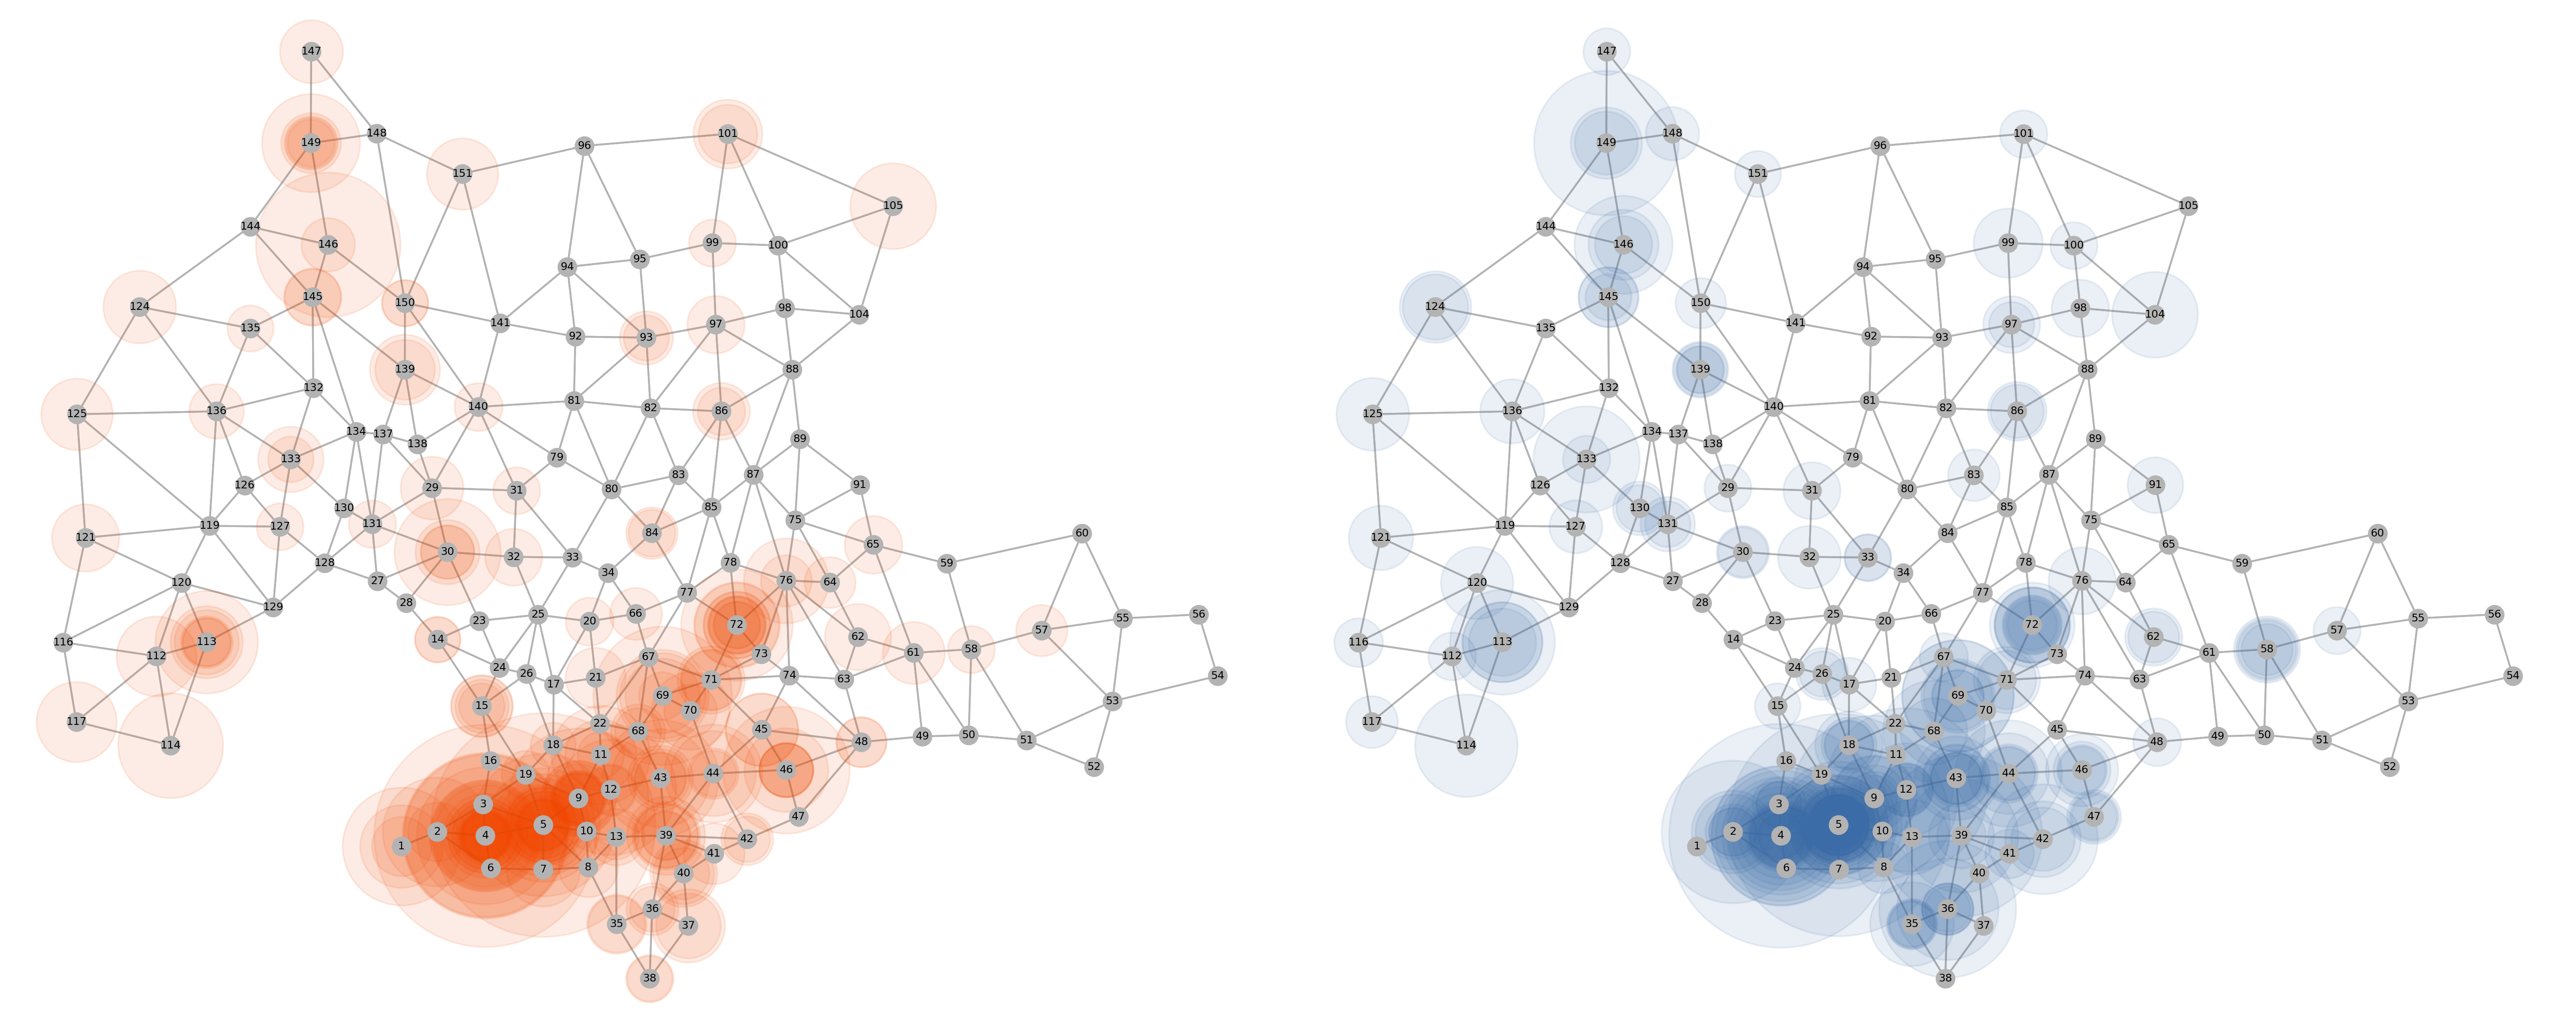
\includegraphics[width=12cm]{../resources/montevideo_demands.png}
    \caption{Representación de los 300 pares origen-destino con más demanda por ubicación de origen y destino. A la izquierda se ubican los orígenes y a la derecha los destinos. Los tamaños de los círculos son proporcionales al valor de demanda y no se suman por nodo. Estos pares origen-destino concentran casi el 60\% de la demanda total de los pares origen-destino considerados.}
  \label{fig:montevideodemanddist}
\end{figure}

Si comparamos las funciones de transferencia de demanda fijando el factor de presupuesto vemos que la lineal induce mayor transferencia y una red de ciclovías que afecta potencialmente a mayor cantidad de demanda por abarcar mayor proporción de la red de calles, ver Tabla \ref{table:montevideoinfracoverage}. Vemos que las ejecuciones con función de transferencia logística utilizaron mayor proporción del presupuesto en tecnologías más caras (Tabla \ref{table:montevideobudgetusage}), lo que lleva a una red de ciclovías más chica en términos de distancia. Por otro lado, si observamos la cantidad de pares origen-destino afectados por instancia vemo que la función logística fue más equitativa al afectar todos los pares origen-destino para todos los factores de presupuesto mientras que las instancias con función de transferencia lineal no lo hizo para ningún caso.

\begin{table}[h!]
  \centering
  \begin{adjustbox}{width=1.2\textwidth,center=\textwidth}
    \begin{tabular}{cccccc}
      \toprule
        Instancia & Presupuesto & \shortstack{Presupuesto \\ utilizado} & Tecn. 1 (\%) & Tecn. 2 (\%) & Tecn. 3 (\%) \\
      \midrule
        1 & 324220.24 & 323559.54 & 1.47 & 34.72 & 63.81 \\
        2 & 324220.24 & 321485.67 & 0.89 & 34.42 & 64.68 \\
        3 & 648440.47 & 647177.53 & 0.42 & 29.77 & 69.8 \\
        4 & 648440.47 & 647883.38 & 1.37 & 31.2 & 67.42 \\
        5 & 1296880.95 & 1296483.25 & 0.65 & 12.02 & 87.33 \\
        6 & 1296880.95 & 1296757.67 & 0.87 & 15.95 & 83.18 \\
      \bottomrule
    \end{tabular}
  \end{adjustbox}
  \caption{Porcentaje del presupuesto utilizado por tipo de tecnología para cada instancia. Debido al redondeo y que el presupuesto no fue utilizado completamente en ninguna instancia los porcentajes no suma 100\%.}\label{table:montevideobudgetusage}
\end{table}

\begin{table}[h!]
  \centering
  \begin{tabular}{ccccc}
    \toprule
      Instancia & Tecn. 1 (\%) & Tecn. 2 (\%) & Tecn. 3 (\%) & Total (\%) \\
    \midrule
      1 & 0,39 & 5,57 & 7,11 & 13,07 \\
      2 &      & 0,69 & 9,65 & 10,34 \\
      3 & 0,65 & 11,21 & 14,22 & 26,09 \\
      4 & 0,33 & 1,22 & 19,30 & 20,86 \\
      5 &      & 9,95 & 35,01 & 44,96 \\
      6 & 0,21 & 2,07 & 38,90 & 41,19 \\
    \bottomrule
  \end{tabular}
  \caption{Proporción del largo total de la red de calles por cada tipo de tecnología.}
  \label{table:montevideoinfracoverage}
\end{table}

\begin{figure}[h!]
  \centering
  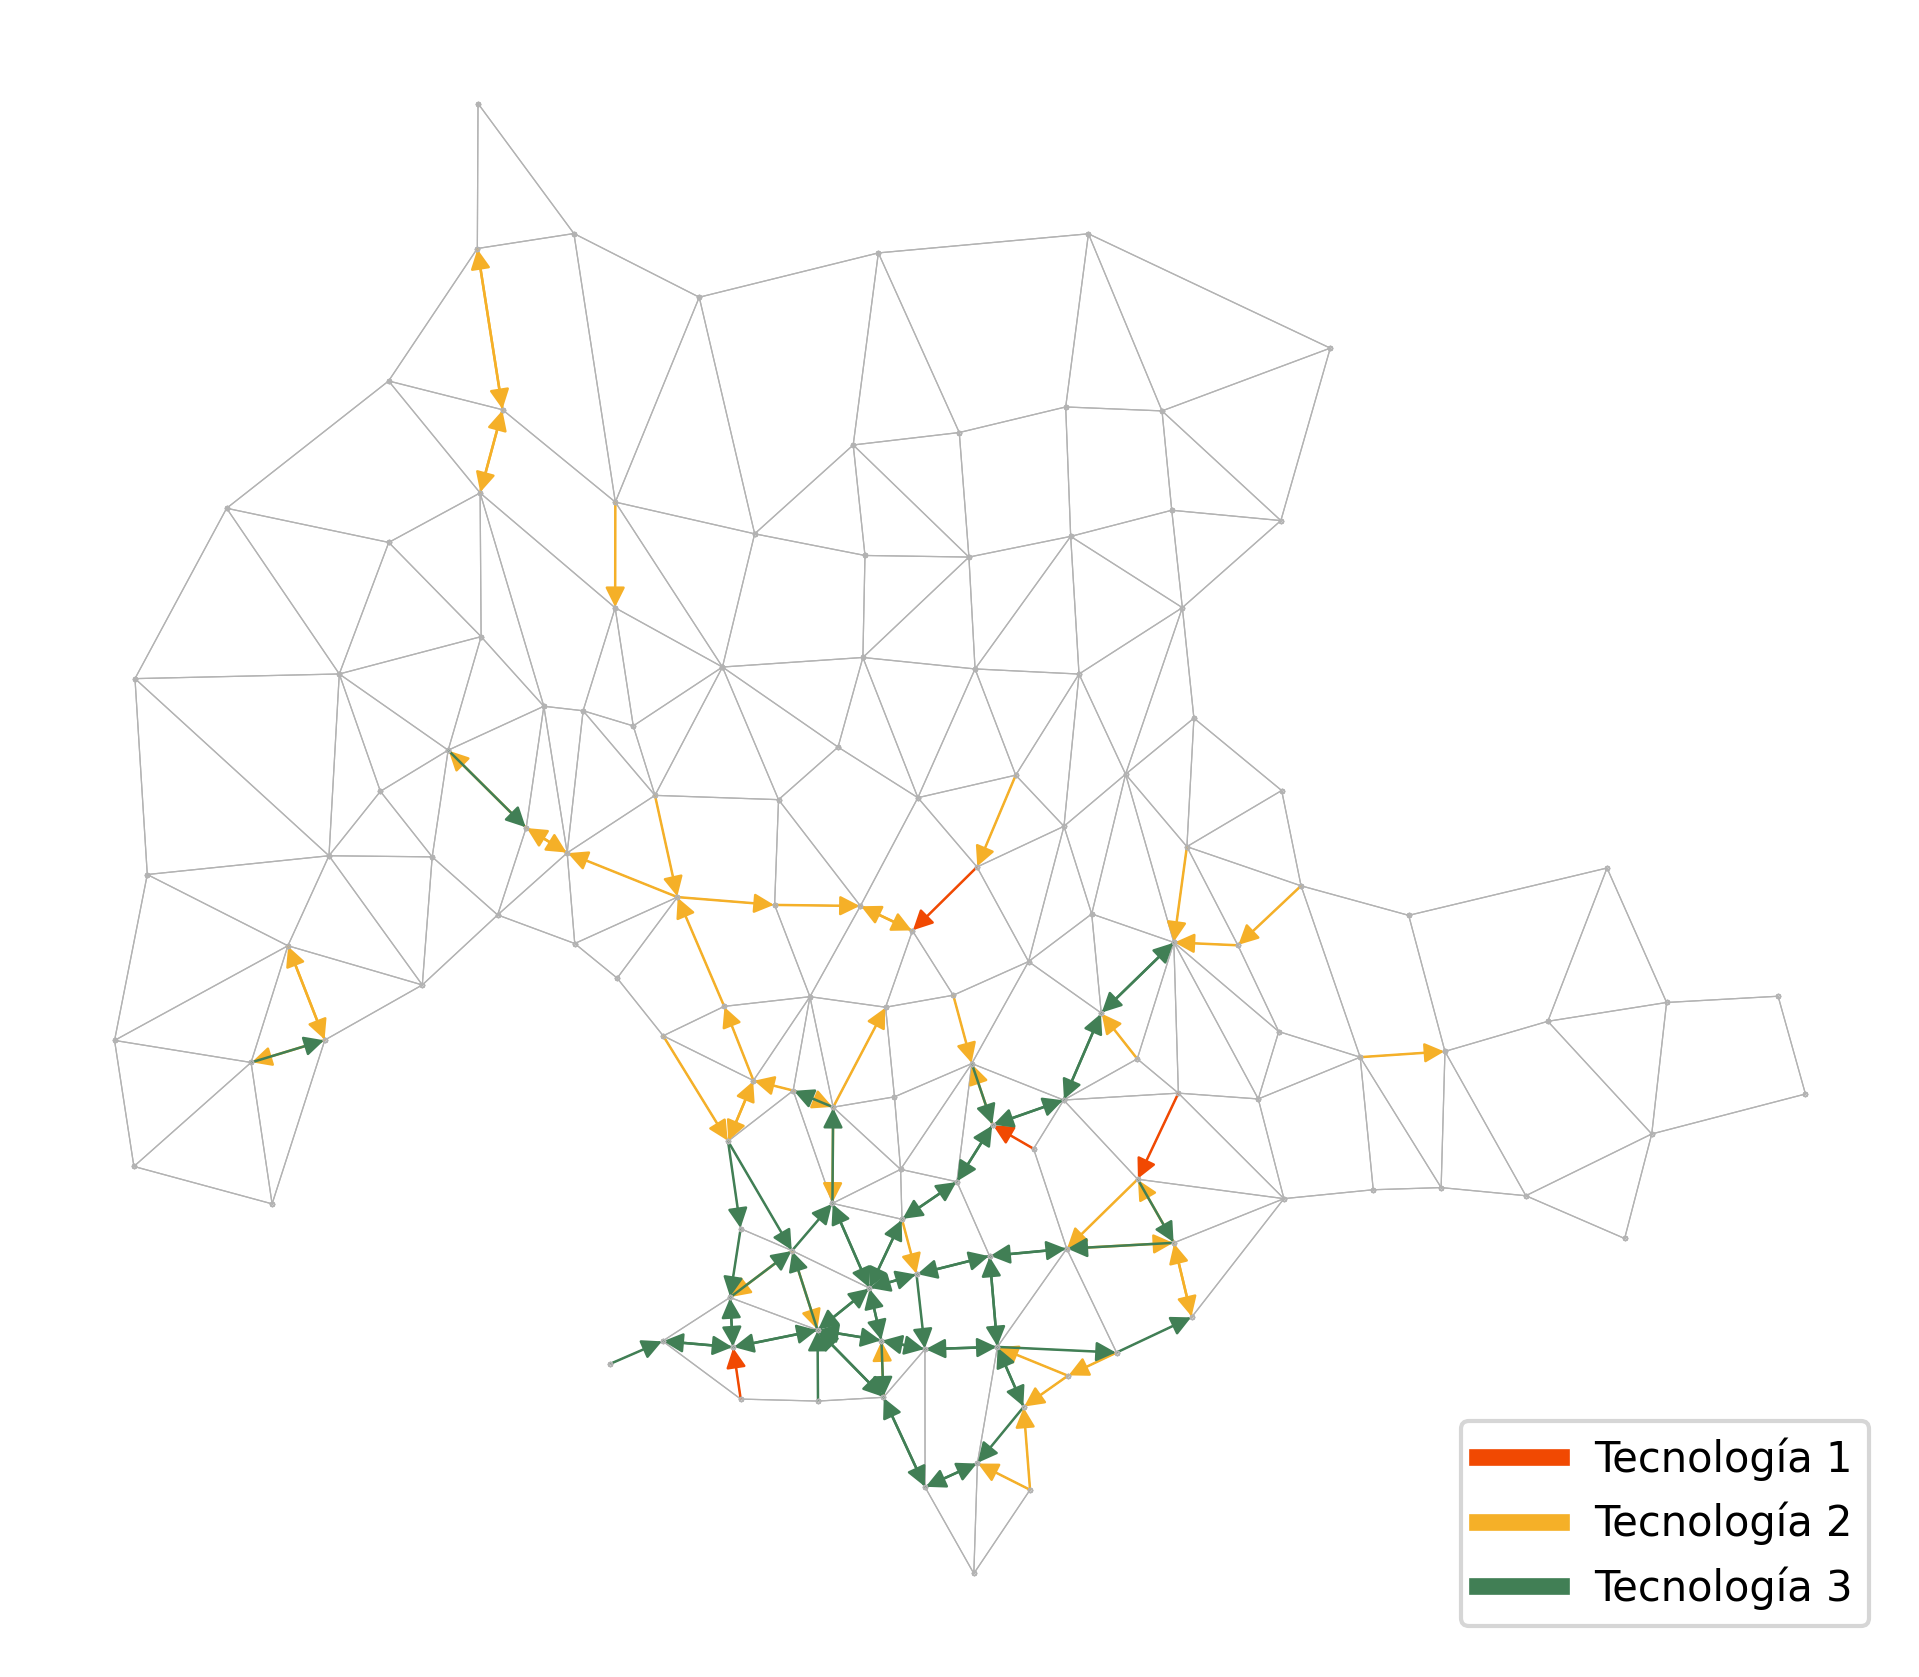
\includegraphics[width=6cm]{../resources/montevideo_d5000.0_linear_0.4_budget_factor.png}
  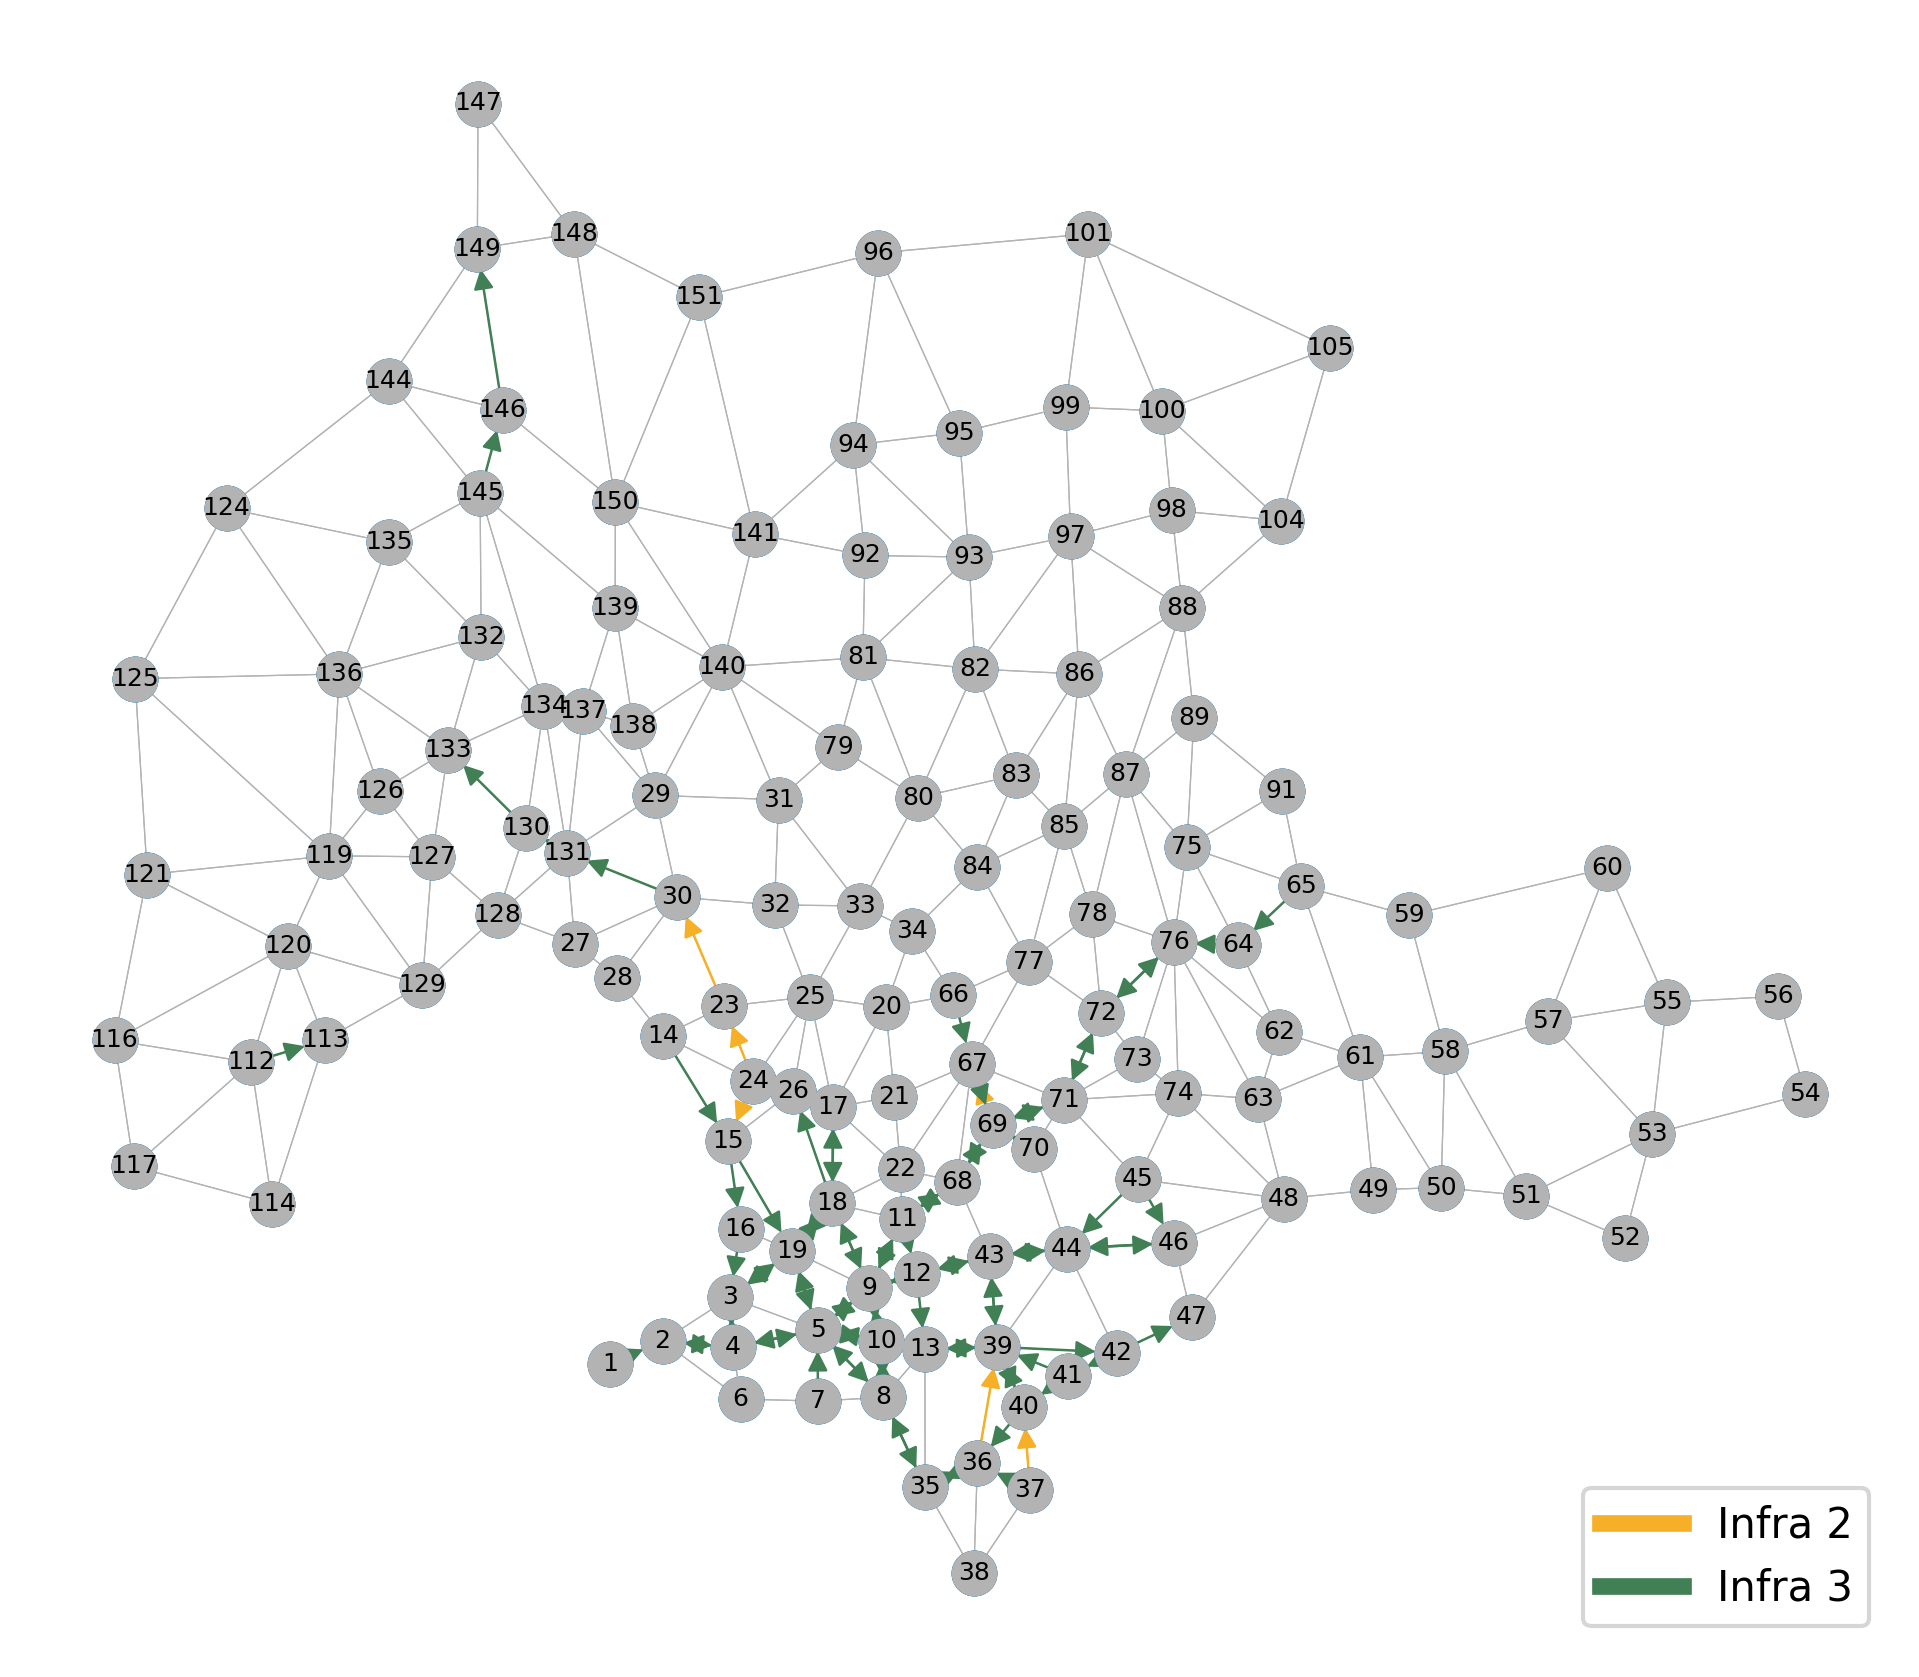
\includegraphics[width=6cm]{../resources/montevideo_d5000.0_inv_logit_0.4_budget_factor.png}
  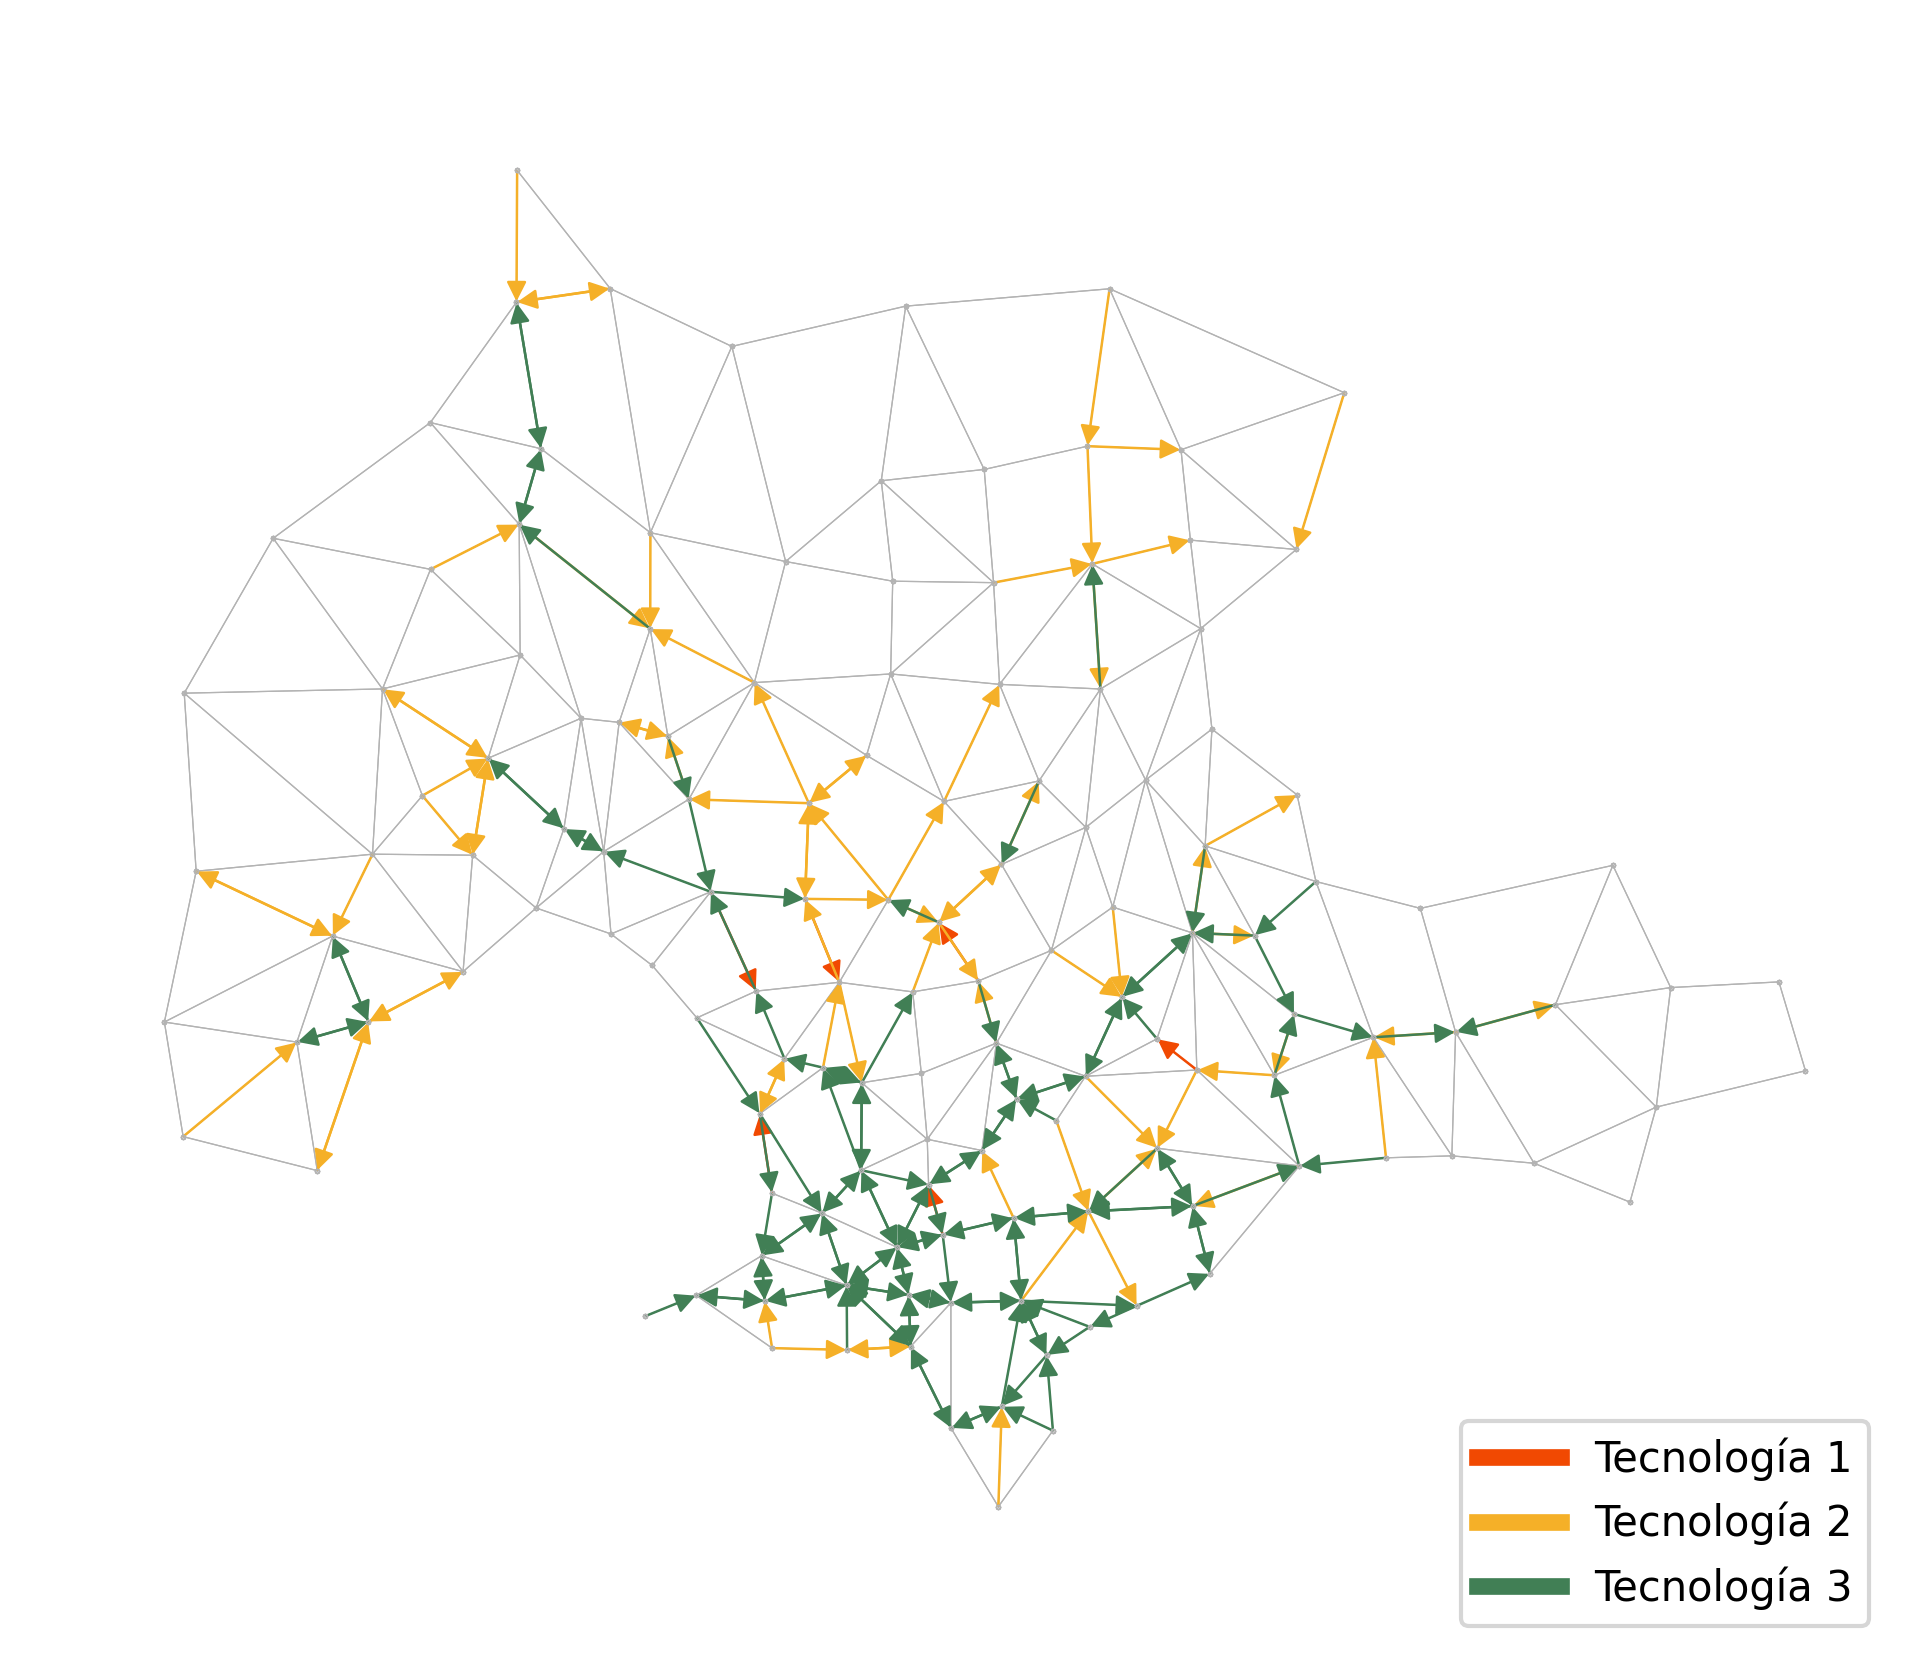
\includegraphics[width=6cm]{../resources/montevideo_d5000.0_linear.png}
  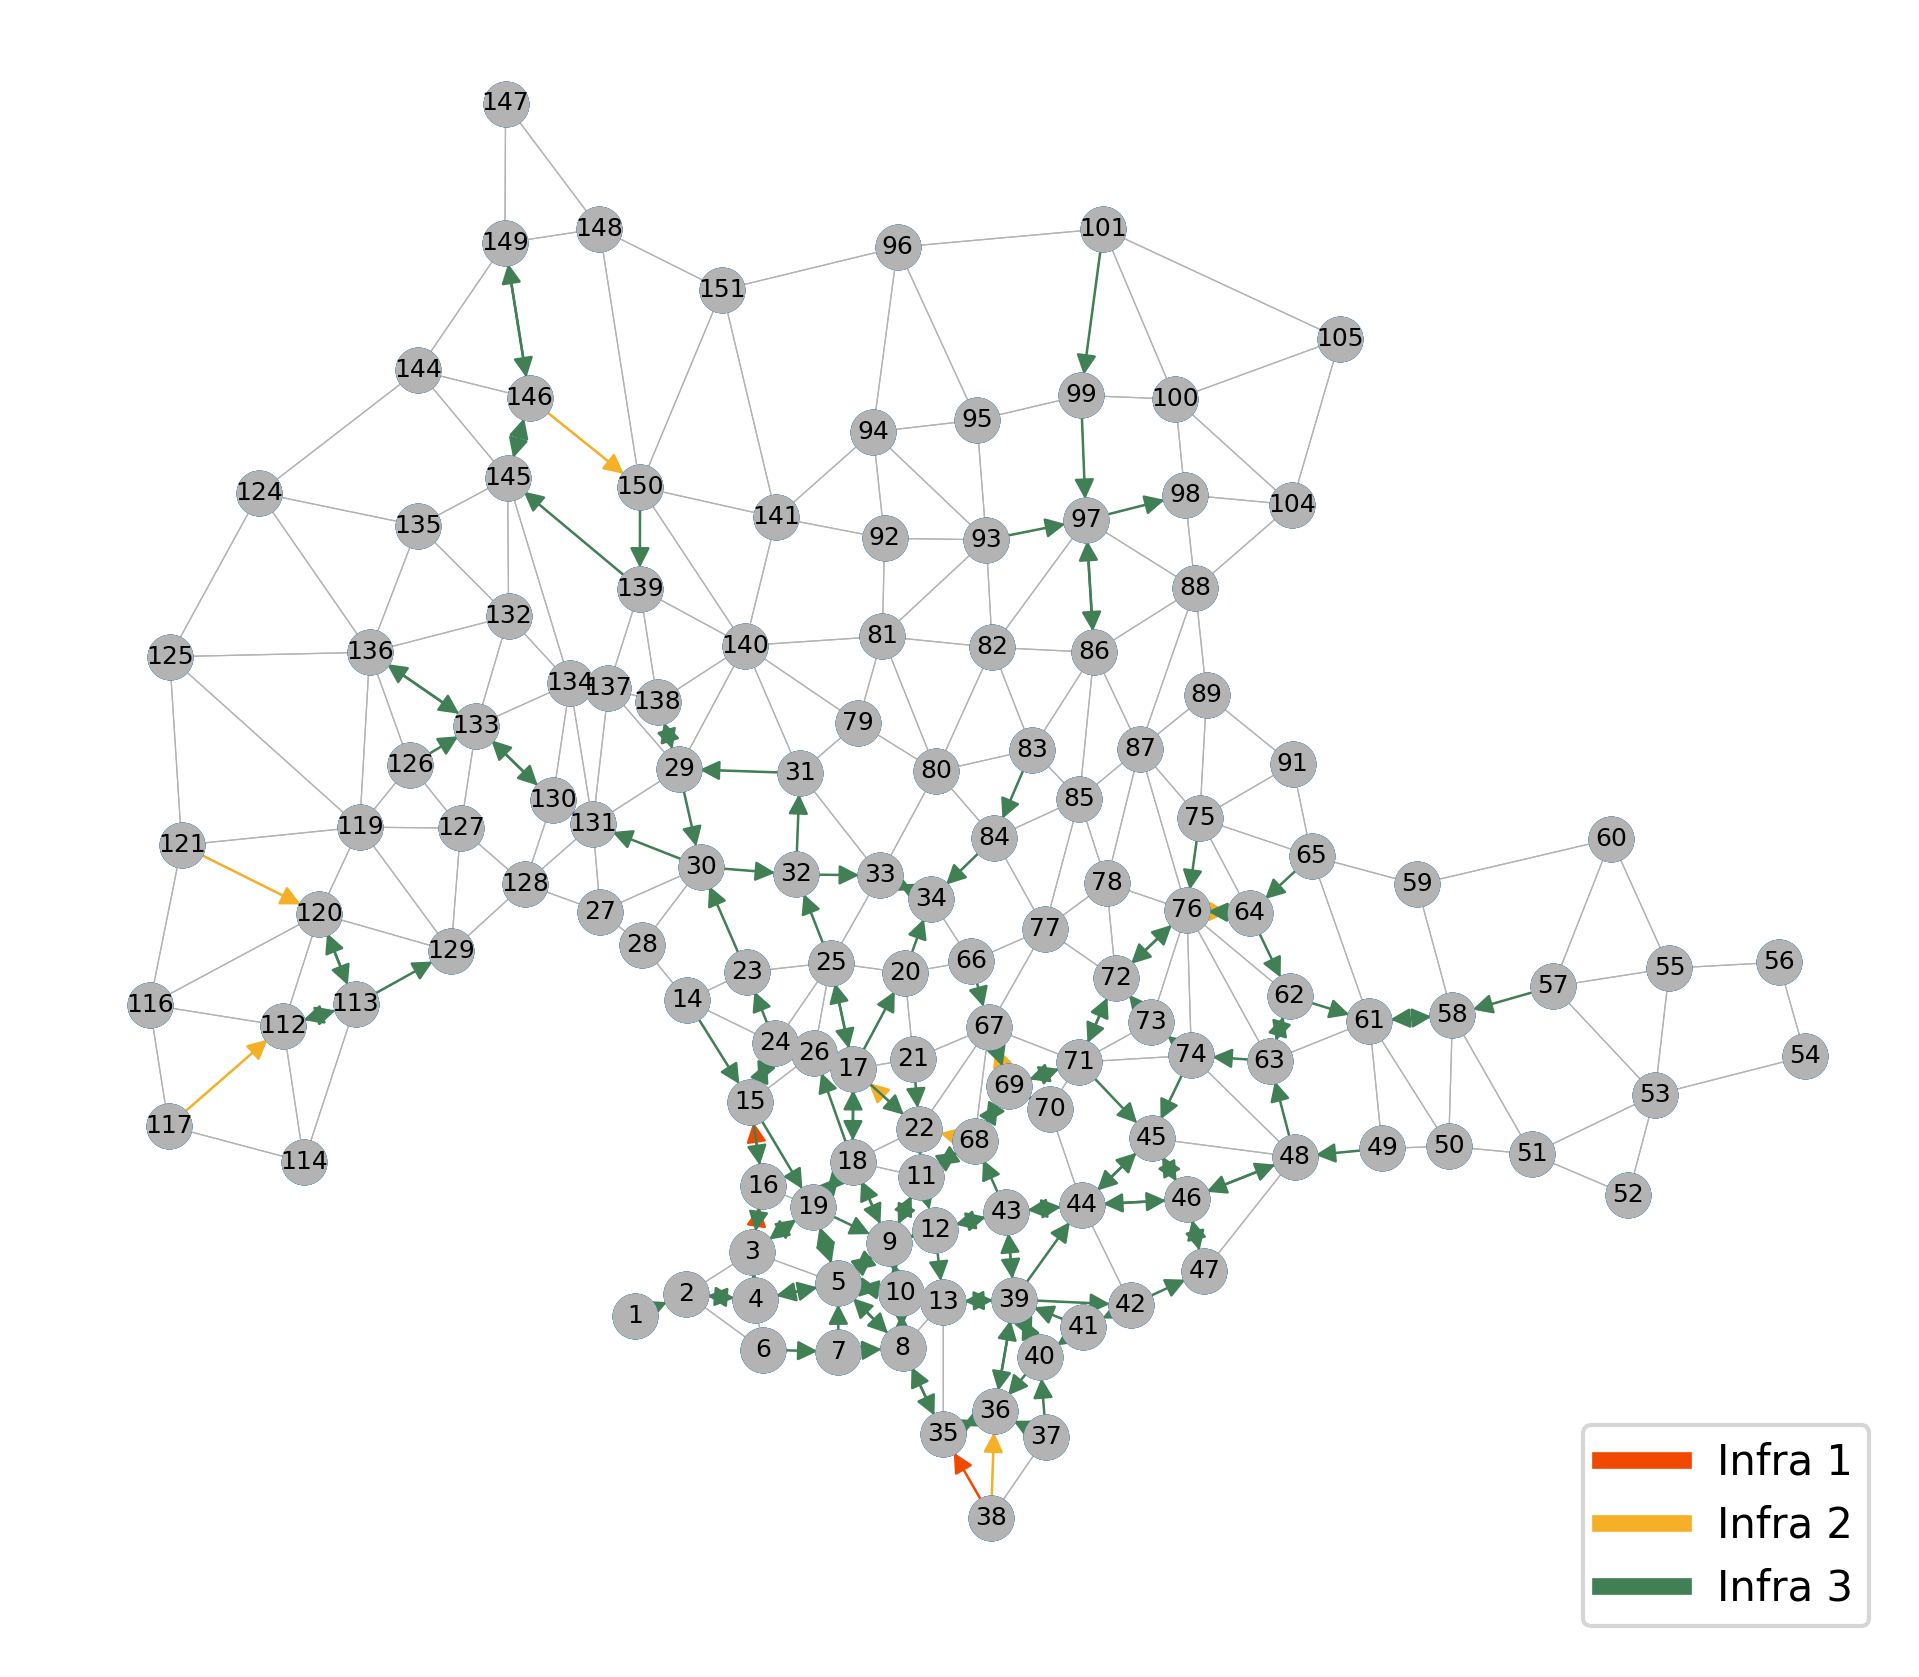
\includegraphics[width=6cm]{../resources/montevideo_d5000.0_inv_logit.png}
  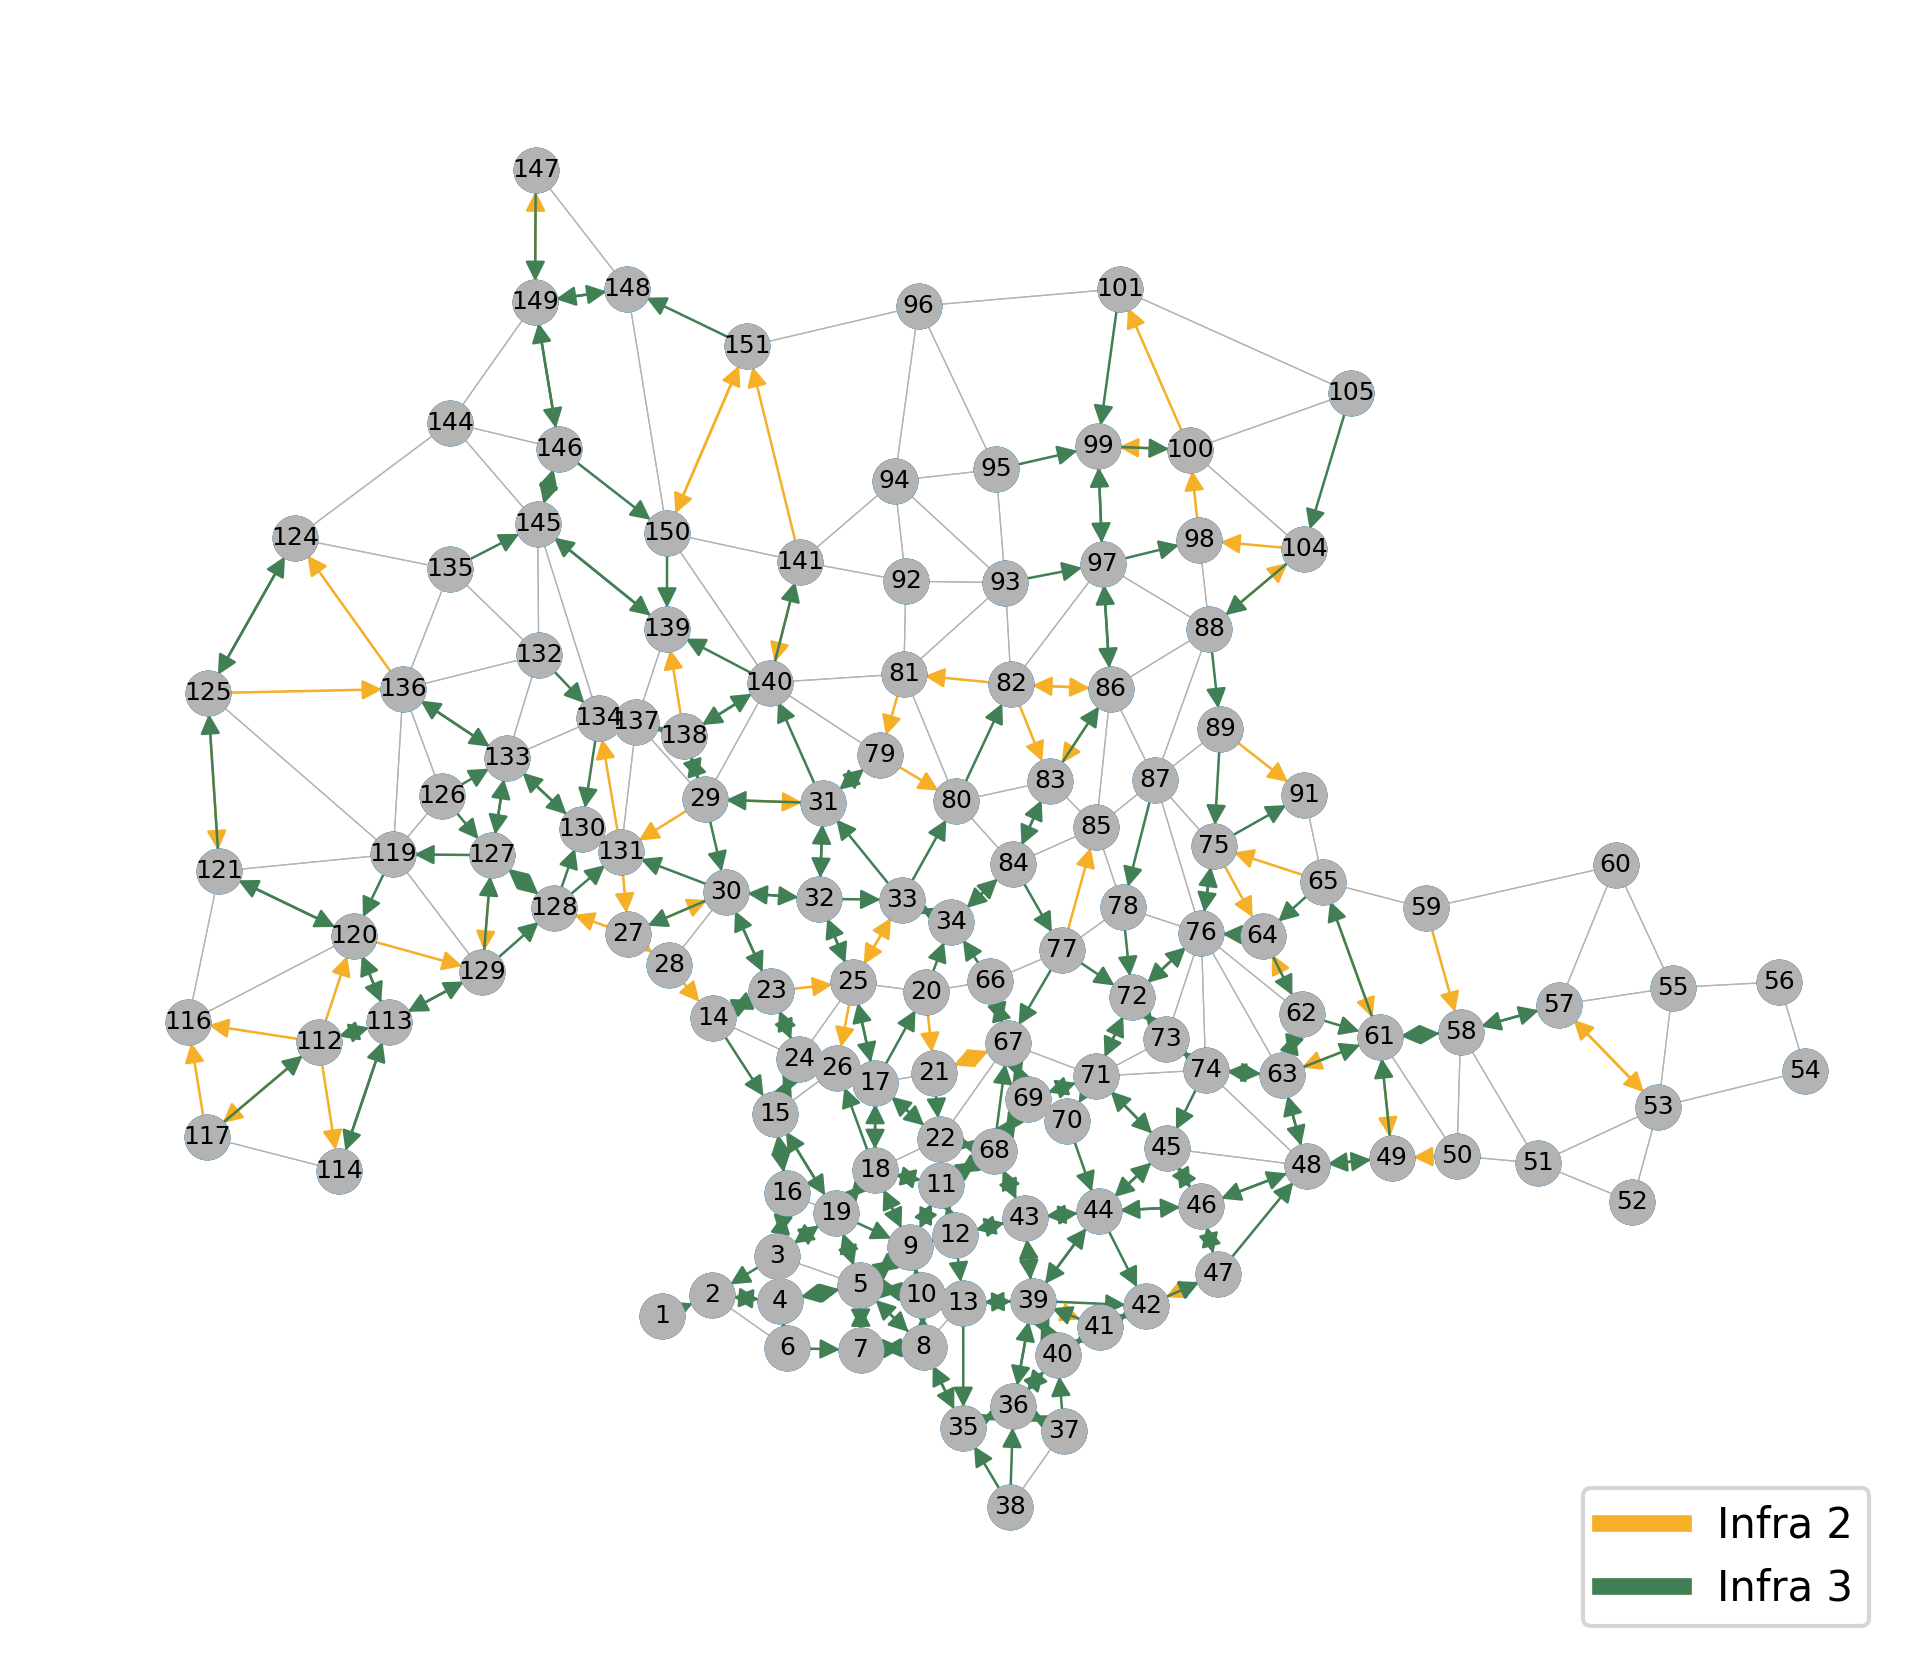
\includegraphics[width=6cm]{../resources/montevideo_d5000.0_linear_1.6_budget_factor.png}
  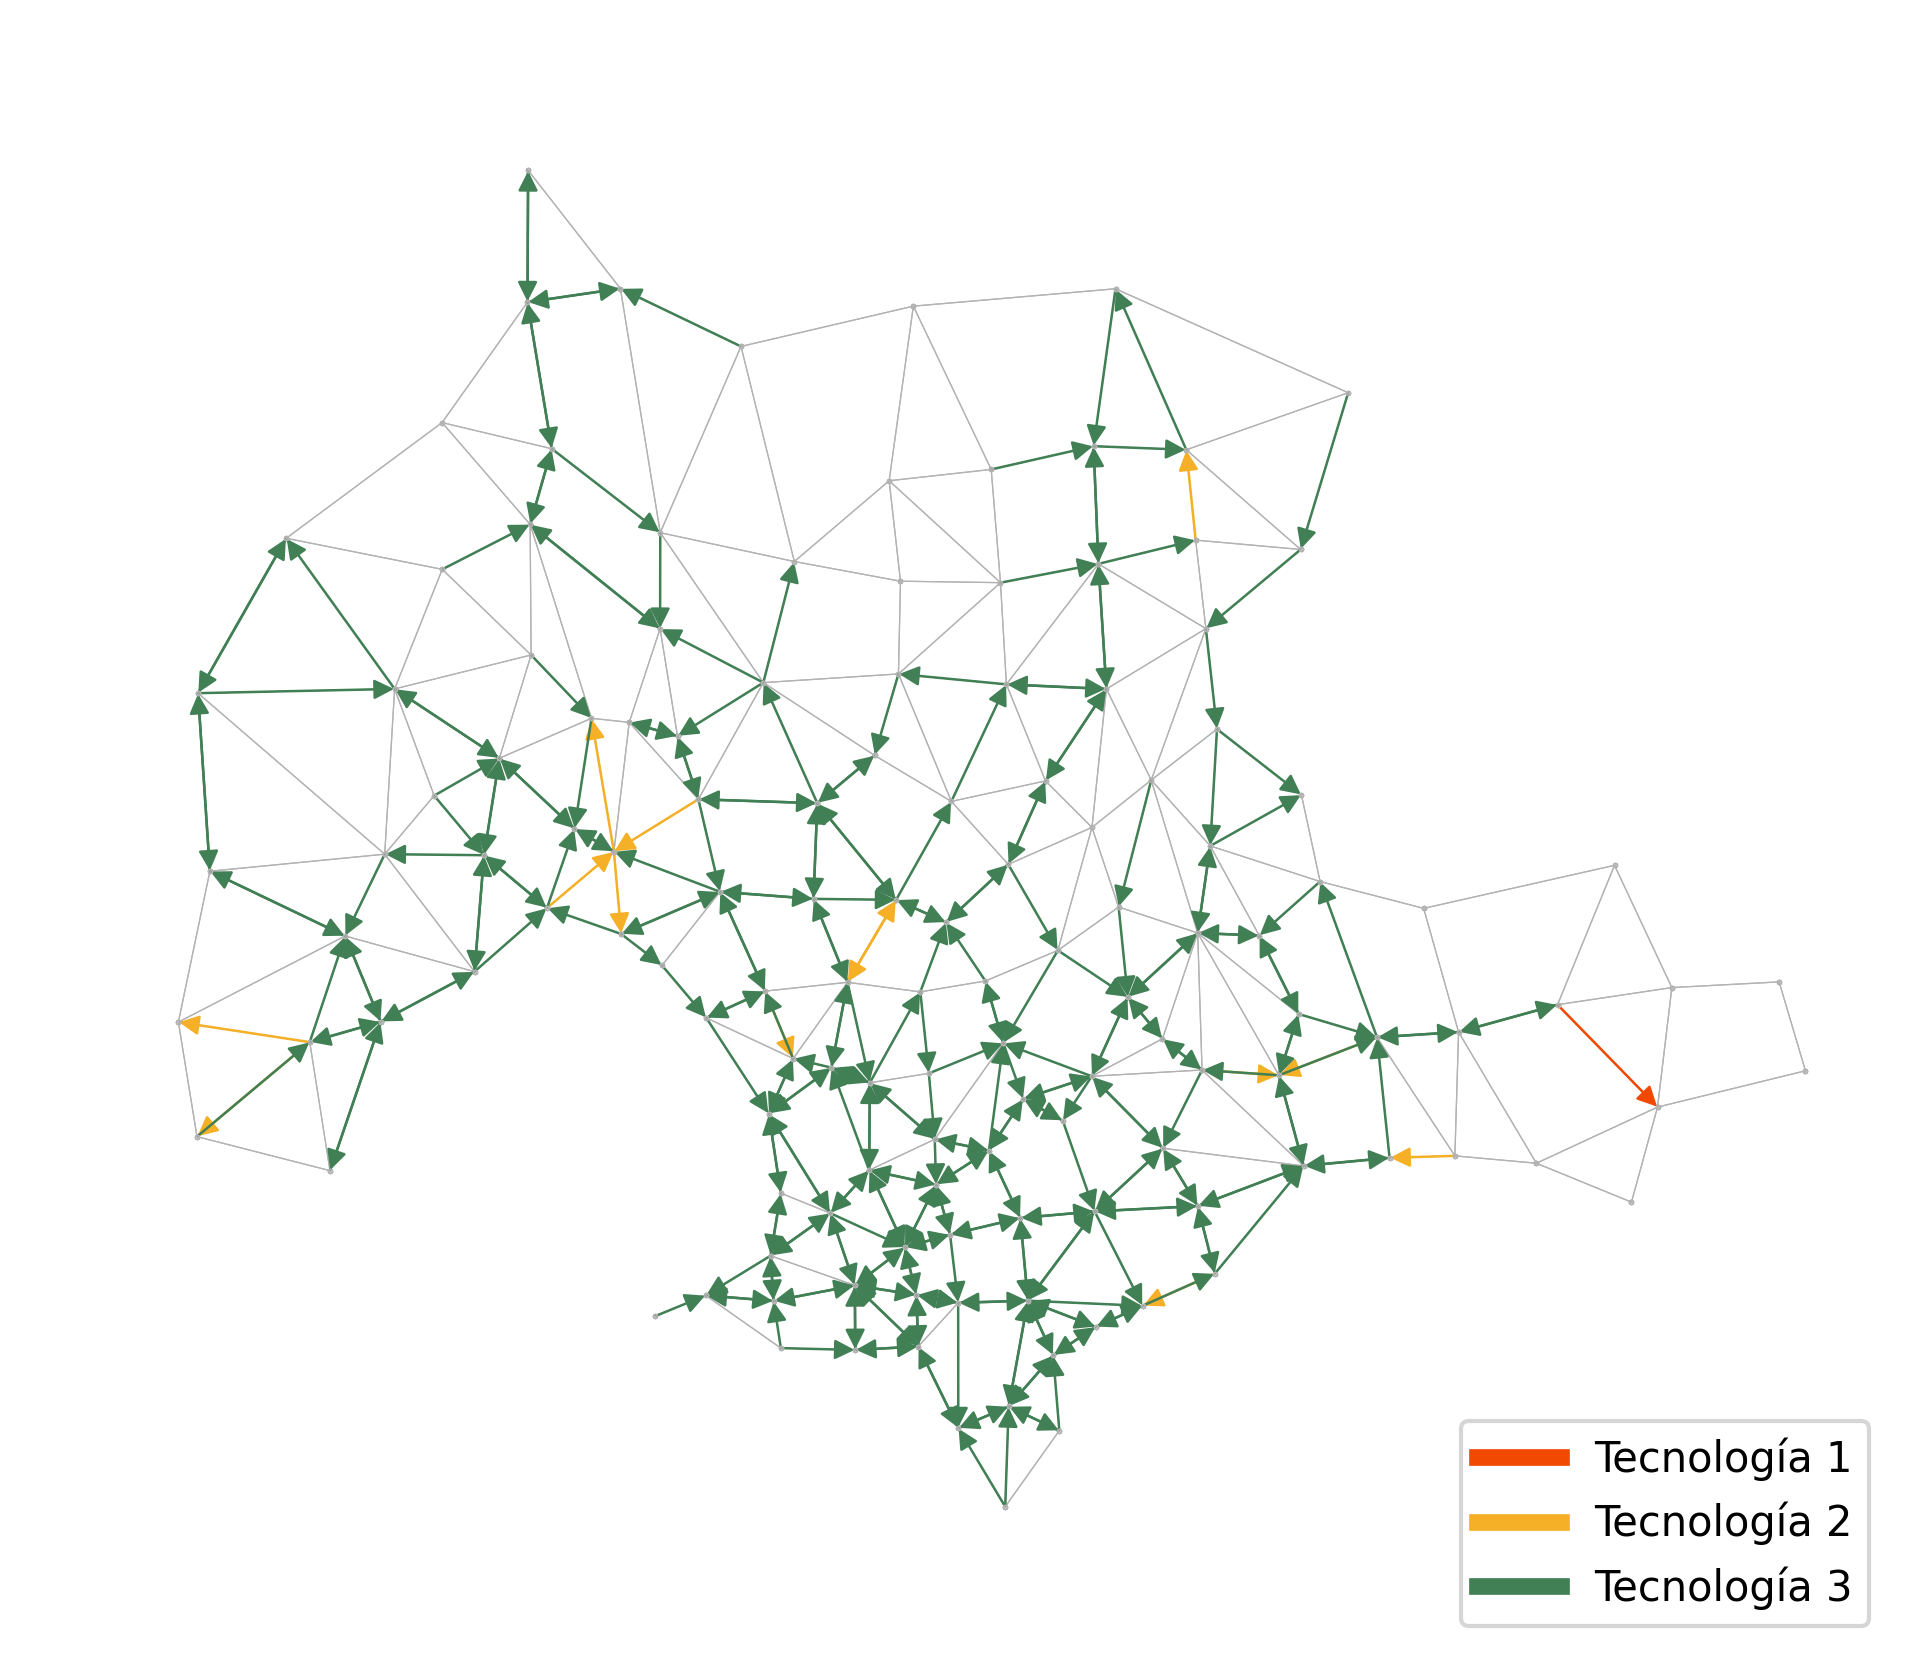
\includegraphics[width=6cm]{../resources/montevideo_d5000.0_inv_logit_1.6_budget_factor.png}
  \caption{Infraestructura de ciclovía construida para cada instancia. A la izquierda se ubican aquellas con función de transferencia de demanda lineal, a la derecha las que utilizan función logística. Además están dispuestas en orden creciente de factor de presupuesto desde arriba.}
  \label{fig:montevideo_instances_infras}
\end{figure}

Como análisis final, comparamos el desvío de los ciclistas respecto al camino más corto en distancia. Recordamos que en \cite{winters2010} el 75\% de los viajes en bici se desvían a lo sumo un 10\% del camino más corto y un 90\% se desvían hasta un 25\%. En nuestras instancias el desvío es menor y no podemos detectar ningún patron específico a menos de un aparente achatamiento de la curva de proporción de desvío hacia las instancias con mayor presupuesto asignado.

\begin{table}[h!]
  \centering
  \begin{tabular}{ccccccc}
    \toprule
      Instancia & 75\% & 90\% & 95\% & 98\% & Máximo \\
    \midrule
      1 & 1.0 & 1.01 & 1.08 & 1.14 & 1.43 \\
      2 & 1.0 & 1.00 & 1.06 & 1.10 & 1.43 \\
      3 & 1.0 & 1.02 & 1.09 & 1.15 & 1.43 \\
      4 & 1.0 & 1.00 & 1.08 & 1.11 & 1.56 \\
      5 & 1.0 & 1.00 & 1.04 & 1.09 & 1.44 \\
      6 & 1.0 & 1.00 & 1.02 & 1.08 & 1.50 \\
    \bottomrule
  \end{tabular}
  \caption{Proporción de desvío sobre el camino más corto en distancia para cada instancia con percentiles por cantidad de demanda. El cálculo se hizo considerando los pares origen-destino para los cuales hay demanda transferida, ordenandolos por factor de desvío y calculando los percentiles por cantidad de viajes sobre la demanda transferida total. Por lo tanto es la misma medida que \cite{winters2010}.}
  \label{table:montevideoshortestpathdeviation}
\end{table}
